\documentclass[acmtocl]{acmsmall}

\usepackage{hyperref}
\usepackage{tikz}
\usetikzlibrary{decorations.markings}
\usetikzlibrary{arrows}
\usepackage{amssymb}
\usepackage{amsfonts,amsmath,latexsym,stmaryrd}
\usepackage{listings}
\usepackage{cite}
\newcommand{\Coq}{{\sc Coq}}
\newcommand{\ssr}{{\sc SSReflect}}
\newcommand{\C}[1]{\mbox{\lstinline`#1`}}
\newcommand\N[1]{\langle\mbox{\itshape\rmfamily\small #1}\rangle}
\newcommand{\iitem}{{\it i-item}}
\newcommand{\ditem}{{\it d-item}}

\let\L=\lstinline

\definecolor{dkblue}{rgb}{0,0.1,0.5}
\definecolor{lightblue}{rgb}{0,0.5,0.5}
\definecolor{dkgreen}{rgb}{0,0.4,0}
\definecolor{dk2green}{rgb}{0.4,0,0}
\definecolor{dkviolet}{rgb}{0.6,0,0.8}
\definecolor{shadethmcolor}{rgb}{0.9, 0.9,1}


\def\lstlanguagefiles{defManSSR.tex}
\lstset{language=SSR}

\lstset{moredelim=[is][\color{red}\bfseries\ttfamily\underbar]{|*}{*|}}
%Highlights metalevel expressions in italic rm font
\lstset{moredelim=*[is][\itshape\rmfamily]{/*}{*/}}

\usepackage{alltt}
\usepackage[all]{xy}
\usepackage{verbatim}
\usepackage{rotating}
\usepackage{pdflscape}
\usepackage{booktabs}
\usetikzlibrary{shapes,snakes}
\newtheorem{PS}[theorem]{Proof Strategy}
\newtheorem{PEM}[theorem]{Proof Exploration Method}




\begin{document}

\markboth{J. Heras and E. Komendantskaya}{Proof-Pattern Search in Coq/SSReflect}

\title{Proof-Pattern Search in Coq/SSReflect}

%                                     also used for the TOC unless
%                                     \toctitle is used
%
\author{J\'onathan Heras
\affil{Department of Mathematics and Computer Science, University of La Rioja, Spain}
Ekaterina Komendantskaya
\affil{School of Computing, University of Dundee, UK}
}




\begin{abstract}
ML4PG is an extension of the Proof General interface, allowing
the user to invoke machine-learning algorithms and find proof similarities
in Coq/SSReflect libraries. In this paper, we present four new improvements to
ML4PG.
First, a new method of \lq\lq{}recurrent clustering" is introduced to collect statistical features from Coq terms.
Now, the user can receive suggestions about similar definitions,
types and lemma statements, in addition to proof strategies. Second, Coq
proofs are split into patches to capture proof strategies that could arise
at different stages of a proof. Third, we present a method to automatically generate Coq proofs based on ML4PG's output. Finally,
we introduce several visualisation tools that help to interpret the families of similar theorems/terms generated by ML4PG.
\end{abstract}



\category{F.4.1}{Mathematical Logic and Formal Languages}{Mathematical Logic -- Mechanical theorem proving}
\category{D.2.4}{Software Engineering}{Software/Program Verification -- Formal methods.}

\terms{}

\keywords{Coq/SSReflect, Proof Patterns, Recurrent Clustering, Pattern Recognition, Feature Extraction.}


\acmformat{J\'onathan Heras and Ekaterina Komendantskaya, 2014.
Proof-Pattern Search in Coq/SSReflect.}


\begin{bottomstuff}
The work was supported by EPSRC grants EP/J014222/1 and EP/K031864/1.

Author's addresses: J\'onathan Heras and Ekaterina Komendantskaya,
School of Computing, University of Dundee, UK
\end{bottomstuff}

\maketitle




\section{Introduction}\label{sec:introduction}


Development of Interactive Theorem Provers (ITPs) has led to the creation of big libraries and varied infrastructures for formal
mathematical proofs.
These frameworks usually involve thousands of definitions and theorems (for instance, there are approximately
4200 definitions and 15000 theorems in the formalisation of the Feit-Thompson theorem~\cite{FTT}).
Parts of  those libraries can often be re-applied in new domains; however,
it is a challenge for expert and non-expert users alike to trace them, and find re-usable concepts and proof ideas.

The ML4PG (``Machine-Learning for Proof-General'') tool~\cite{KHG13,CICM13,HK14} was created to help the user in such a situation for the particular case of the Coq system~\cite{Coq} and its SSReflect extension~\cite{SSReflect} developments. ML4PG uses statistical machine-learning algorithms to discover re-usable proof-patterns based on ``previous experience'' acquired from previous developments. A proof-pattern was defined as a correlation between the tactics and the types/shapes of subgoals resulting from the tactic applications within a few proof steps. The resulting tool could indeed find some interesting --- unexpected and yet relevant --- proof-patterns,
across different notation, types, and libraries. Our experiments spanned several subjects: basic mathematical infrastructures, Computer Algebra, Game Theory, and the certification of Java-like bytecode. The results are best summarised in~\cite{CICM13,HK14}.

That initial approach had two inherent limitations. First, the essence of a Coq/SSReflect proof is not fully expressible by a sequence of applied tactics. The definitions, types, and shapes of auxiliary lemmas used in a proof can be much more sophisticated and conceptual than a proof script calling them. Therefore, although ML4PG could find interesting, and often useful, sequences of tactics; it could not go further to recognise, for instance, similar definitions. Second, the notion of a proof-pattern being ``interesting'' or useful is left to the user's judgement.

In this paper, we present the most recent extensions to ML4PG  involving all kinds of Coq terms --- type declarations, definitions and lemma statements --- into the process of proof-pattern search. This required additional algorithms of feature extraction that reflect the mutual dependency of various proof objects in Coq\rq{}s dependently-typed setting; see Sections~\ref{sec:lemmaclustering} and~\ref{sec:reclemmaclustering}.
This major step in ML4PG development prompted other improvements. The initial ML4PG was considering features arising from the first 5 proof-steps in a proof, whereas now we treat every proof as a collection of
proof patches, each potentially
representing an interesting proof strategy. Moreover, if say 15th-20th step in one proof resembles a 115th-120th step in another, the tool is now able to detect such patterns deep down.
The feature extraction algorithms for proof features have been further refined to include the data collected from Coq terms, and now the
whole syntax of the chosen proof libraries is subject
to \emph{recurrent clustering} --- a novel technique for ML4PG.
All these extensions to proof-feature extraction are explained in Section~\ref{sec:recurrent}.

ML4PG used to show, in response to the user's call, a set of similar proofs,
with no hints of why these proofs are deemed similar. We now introduce two extensions that improve ML4PG's user-experience.
First, we have designed a method to automatically proof theorems based on ML4PG clustering methods (cf. Section~\ref{sec:evaluation}). Additionally, several visualisation tools (using automaton-shape or tree-shape representations) have been developed to show the proof-features that correlate, see Section~\ref{sec:visualisation}. This partially addresses the drawback of the subjective approach to
the pattern's ``interestingness'' --- now
the tool clearly declares correlation of which proof features defined the suggested proof pattern.
Finally, in Section~\ref{sec:relatedwork}, we compare ML4PG with other machine-learning and searching approaches available in the literature, and conclude the paper in Section~\ref{sec:conclusions}.


Examples we use throughout the paper come from several Coq and SSReflect libraries: the basic infrastructure of SSReflect~\cite{SSReflect}, a matrix library~\cite{GarillotEtAl09}, a formalisation of persistent homology~\cite{HCMS12}, the HoTT library~\cite{hottbook}, two formalisation related to Nash equilibrium~\cite{Ves06,nash}, and the formalisation about Java-like bytecode presented in~\cite{HK14}. ML4PG is a part of standard Proof General distribution; the novel features we present here are available at~\cite{HK12}.


\section{Feature Extraction for Coq terms}\label{sec:lemmaclustering}

ML4PG uses (unsupervised) \emph{clustering algorithms}~\cite{Bishop} to find patterns in Coq syntax and proofs.
Clustering algorithms % is a set of machine-learning techniques that 
divide data into $n$ groups of similar objects (called \emph{clusters}), where the value of $n$
is a parameter provided by the user. In ML4PG, the value of $n$ is automatically computed depending on the number 
of objects to cluster, and using the formula provided in~\cite{KHG13,lpar13}. 
A detailed exposition of machine-learning algorithms involved in ML4PG can be found in \cite{KHG13}. In this paper, our first goal consists in improving ML4PG's feature extraction algorithm.
%In this section, we present a method to collect features from Coq terms. 


\emph{Feature extraction}~\cite{Bishop} is a research area developing methods for 
discovery of statistically significant features in data. % in machine-learning, known as . 
We adopt the following standard terminology. % concerning feature extraction. 
We assume there is a training data set, containing some samples (or objects). 
\emph{Features} are given by a set of statistical parameters chosen to represent all objects in the given data set.
If $n$ features are chosen, one says that object classification is 
conducted in an $n$-dimensional space. 
For this reason, most pattern-recognition tools will require that %the features have numeric values; and 
the number of selected features is limited and fixed (sparse methods, like the ones applied in
e.g.~\cite{lpar-urban,K13,UrbanSPV08} are the exception to this rule). 
\emph{Feature values} are rational numbers used to instantiate the features for every given object.  
If an object is characterised by $n$ feature values, these $n$ values together form a \emph{feature vector} for this object. 
%Irrespective of the particular algorithm
%used, 
A function that assigns, to every object of the data set, a feature vector is called a \emph{feature extraction function}.
Normally, feature extraction is a data pre-processing stage, and it is separated from the actual pattern-recognition process. %ML4PG relies on unsupervised clustering methods~\cite{KHG13}.


Feature extraction from terms or \emph{term trees} is common to most feature extraction algorithms implemented
in theorem provers~\cite{lpar13,lpar-urban,K13,UrbanSPV08}. In~\cite{lpar13}, we introduced a feature extraction mechanism
for ACL2 first-order terms. Here, that ACL2 method is substantially re-defined to capture the higher-order dependently-typed language of Coq.
%However, due to the different nature of ACL2 and Coq -- ACL2 being a first-order untyped language, and Coq being a higher-order
%dependently-typed language -- the algorithm presented in~\cite{lpar13} cannot be extrapolated to Coq, and a different method is necessary.
%Therefore, we introduce here a new feature-extraction method for Coq terms.



The underlying formal language of Coq is known as the \emph{Predicative Calculus of (Co)Inductive Constructions} (pCIC)~\cite{Coq,CoquandH88,CoPa89}. % -- a 
%weaker calculus of the \emph{Calculus of (Co)Inductive Constructions}. 
The terms of pCIC are built from
the following rules:


\begin{definition}[pCIC term]\label{def:coqterms}

$-$ The sorts \lstinline?Set?, \lstinline?Prop?, \lstinline?Type(i)? (\lstinline?i?$\in \mathbb{N}$) are terms.

$-$ The global names of the environment are terms. 

$-$ Variables are terms.
 
$-$ If \lstinline?x? is a variable and \lstinline?T, U? are terms, then \lstinline?forall x:T,U? 
 is a term. If \lstinline?x? does not occur in \lstinline?U?, then \lstinline?forall x:T,U? will be written as \lstinline?T -> U?. A term of the 
 form \lstinline?forall x1:T1, forall x2:T2, ..., forall xn:Tn, U? will be written as \lstinline?forall (x1:T1) (x2:T2) ...(xn:Tn), U?. 
 
$-$ If \lstinline?x? is a variable and \lstinline?T, U? are terms, then \lstinline?fun x:T => U? 
 is a term. A term of the form \lstinline?fun x1:T1 => fun x2:T2 => ... => fun xn:Tn => U? will be written as \lstinline?fun (x1:T1) (x2:T2) ...(xn:Tn) => U?. 

 $-$ If \lstinline?T? and \lstinline?U? are terms, then \lstinline?(T U)? is a term -- we use an uncurried notation (\lstinline?(T U1 U2 ... Un)?) 
 for nested applications (\lstinline?(((T U1) U2) ... Un)?).
 
 $-$ If \lstinline?x? is a variable, and \lstinline?T, U? are terms, then (\lstinline?let x:=T in U?) is a term.

\end{definition}

The syntax of Coq terms~\cite{Coq} includes some terms that do not appear in Definition~\ref{def:coqterms}; e.g. given 
 a variable \lstinline?x?, and  terms \lstinline?T? and \lstinline?U?, \lstinline?fix name (x:T) := U? is a Coq term used to declare a recursive definition.
The notion of a term in Coq covers a very general syntactic
category in the Gallina specification language~\cite{Coq} and corresponds to the intuitive notion of well-formed expression. 
%Our feature extraction
%method works for all well-formed expressions that can be defined in Coq; 
However, for the purpose of concise exposition, % purposes,
we will restrict our notion of a term to Definition~\ref{def:coqterms},
giving the full treatment of the whole Coq syntax in the actual ML4PG implementation.
 % %definitions to the syntax of Coq terms coming from pCIC terms, thereby remembering that full Coq syntax is handled in the actual ML4PG implementation. 


\begin{definition}[ML4PG term tree]\label{def:ml4pgtermtree}
Given a Coq term \lstinline?C?, we define its associated term tree as follows:

$-$ If \lstinline?C? is one of the sorts \lstinline?Set?, \lstinline?Prop? or \lstinline?Type(i)?, then the term tree of 
 \lstinline?C? consists of one single node, labelled respectively by \lstinline?Set:Type(0)?, \lstinline?Prop:Type(0)? or \lstinline?Type(i):Type(i+1)?.
 
$-$ If \lstinline?C? is a name or a variable, then 
 the term tree of \lstinline?C? consists of one single node, labelled by the name or the variable itself together with its type.
 
$-$ If \lstinline?C? is a term of the form \lstinline?forall (x1:T1) (x2:T2) ...(xn:Tn), U? (analogously for \lstinline?fun (x1:T1) (x2:T2) ...(xn:Tn) => U?); 
then, the term tree of \lstinline?C? is the tree with the root node labelled by \lstinline?forall? (respectively \lstinline?fun?) 
and its immediate subtrees given by the trees representing \lstinline?x1:T1?, \lstinline?x2:T2?, \lstinline?xn:Tn? and \lstinline?U?.

$-$ If \lstinline?C? is a term of the form \lstinline?let x:=T in U?, then the term tree of \lstinline?C? 
 is the tree with the root node labelled by \lstinline?let?, having three subtrees given by the trees corresponding to \lstinline?x?, \lstinline?T? and \lstinline?U?.
 
 
$-$ If \lstinline?C? is a term of the form  \lstinline?T -> U?, then  the term tree of \lstinline?C?  is represented by the tree with the root node labelled by 
\lstinline?->?, and its immediate subtrees given by the trees representing  \lstinline?T? and \lstinline?U?.

$-$ If \lstinline?C? is a term of the form  \lstinline?(T U1 ... Un)?, then we have two cases.
If \lstinline?T? is a name, the term tree of \lstinline?C?  is represented by 
the tree with the root node labelled by \lstinline?T? together with its type, and its immediate subtrees given by the trees
representing \lstinline?U1?,\ldots, \lstinline?Un?. If \lstinline?T? is not a  name, the term tree of \lstinline?C?
is the tree with the root node labelled by \lstinline?@?, and its immediate subtrees given by the trees 
representing \lstinline?T?, \lstinline?U1,...,Un?.


\end{definition}


Note that ML4PG term trees consist of two kinds of nodes: \emph{Gallina} and \emph{term-type} nodes. The Gallina nodes are 
labelled by Gallina-keywords and special tokens such as \lstinline?forall?, \lstinline?fun?, \lstinline?let? or \lstinline?->? (from now on, we will call them Gallina tokens); 
%to
%Gallina keywords and special tokens); 
and the term-type nodes are labelled by expressions of the form \lstinline?t1:t2? where \lstinline?t1? is a sort, a variable or 
a name, and  \lstinline?t2? is the type of \lstinline?t1?.  


\begin{figure}[t]
\centering
\begin{tikzpicture}[level 1/.style={sibling distance=40mm},
 level 2/.style={sibling distance=70mm},
 level 3/.style={sibling distance=30mm},
 level 4/.style={sibling distance=30mm},scale=.8,font=\footnotesize]
   
   \node (root) {\lstinline?forall?} [level distance=10mm]
             child { node {\lstinline?n : nat?}}
             child { node {\lstinline?H : even n?}}
             child { node {\lstinline?odd : nat -> Prop?} 
                      child { node {\lstinline?+ : nat -> nat -> nat?}
                           child { node {\lstinline?n : nat?}}
                           child { node {\lstinline?1 : nat?}}
                           }
                   }
            
    ;
 \end{tikzpicture}
\caption{\scriptsize{\emph{ML4PG term tree for the term \texttt{forall (n : nat) (H : even n), odd (n + 1).}}}}\label{fig:termtree}
\end{figure}  

\begin{example}\label{ex1}
 Given the term \lstinline?forall (n : nat) (H : even n), odd (n + 1)?, its ML4PG term tree is depicted in Figure~\ref{fig:termtree}.
 \end{example}

We represent ML4PG term trees as feature matrices, further to be flattened into feature vectors for clustering. %they in turn will be the input of machine-learning algorithms.
A variety of methods exists to represent trees as matrices, for instance using
adjacency or incidence matrices. The adjacency matrix and the various previous methods of  feature
extraction (e.g.~\cite{lpar-urban,K13,UrbanSPV08}) share the following common properties: different %tree
%nodes 
library symbols are represented by distinct features, and the %matrix entries
feature values are binary. %; and the size of the matrix depends on the tree size. 
For
big libraries and growing syntax, feature vectors grow very large (up to $10^6$ in some experiments)
and at the same time very sparse, which implies the use of sparse machine-learning methods. 


%In~\cite{lpar13}, we represent ACL2 term trees as matrices with the following properties: the features are 
%given by the arity of functions and the term tree depth -- two properties common to every term tree -- and the 
%feature values are rational numbers dynamically computed depending on the definition of the functions involved in the term tree. The size of 
%those matrices is fixed to $49$; hence, allowing the application of data-mining techniques to both big and small 
%data sets of ACL2 theorems -- large and sparse feature vectors require to use big data sets, 
%where the size of the example data set is comparable to the number of features; on the contrary, compact feature extraction methods work equally well 
%with both big and small datasets. The method presented in~\cite{lpar13}
%can be applied not only to ACL2 but also to any first-order theory; however, it is not sufficient to capture all the information 
%from the higher-order dependently-typed language of Coq. 


We develop a new compact method that tracks a large (potentially unlimited) number of Coq terms by a finite number of features and an unlimited number of feature-values.
In our method, the features are given by two properties common to all possible term trees: the term tree depth and the level index of nodes.
The most important information about the term is then encoded by improving precision of feature values %means of a more precise specification of feature values, 
using rational-valued feature-extraction functions. Taking just $300$ features, the new feature-extraction method recursively adjusts the feature values, 
adapting to the growing language syntax. %; thus producing a machine-learning analogue of how an unlimited number of Coq terms can be generated from the limited syntactic constructs.  
The resulting feature vectors have an average density ratio of 60\%.   

Given a Coq expression, we can differentiate its term and type components; the feature values capture information from
these components and also the structure of the tree. In particular, each tree node is encoded by distinct feature values
given by a triple of rational numbers to represent the term component, the type component, and the level index of the parent node in the term tree,
cf. Table~\ref{ml4pgtermtable}. Our feature extraction method is formalised in the following definitions.

\begin{table}[t]
\tbl{\scriptsize{\emph{ML4PG term tree matrix for \texttt{forall (n : nat) (H : even n), odd (n+1)}.}}\label{ml4pgtermtable}}{
\centering
{\scriptsize 
\begin{tabular}{|c||c|c|c|}
\hline
 &  level index 0 & level index 1 & level index 2 \\
 \hline
td0 & ($[\texttt{forall}]_{Gallina}$,-1,-1) & (0,0,0) & (0,0,0)\\
\hline
td1 & ($[\texttt{n}]_{term}$,$[\texttt{nat}]_{type}$,0) & ($[\texttt{H}]_{term}$,$[\texttt{even n}]_{type}$,0)& ($[\texttt{odd}]_{term}$,$[\texttt{nat-> Prop}]_{type}$,0) \\
\hline
td2 & ($[\texttt{+}]_{term}$,$[\texttt{nat -> nat -> nat}]_{type}$,2) & (0,0,0)& (0,0,0)\\
\hline
td3 & ($[\texttt{n}]_{term}$,$[\texttt{nat}]_{type}$,0) & ($[\texttt{1}]_{term}$,$[\texttt{nat}]_{type}$,0)  & (0,0,0)\\
\hline
\end{tabular}}}
\end{table}


\begin{definition}[Term tree depth level and level index]\label{def:termtreelevel}
Given  a term tree $T$, the \emph{depth} of the node $t$ in $T$, denoted by \emph{depth(t)}, is defined as follows:

$-$ $depth(t) = 0$, if $t$ is a root node;

$-$ $depth(t) = n+1$, where $n$ is the depth of the parent node of $t$.

The \emph{$n$th level} of $T$ is the ordered sequence of nodes of depth $n$ --- using the classical representation for trees, the order of the sequence is 
given by visiting the nodes of depth $n$ from left to right. The \emph{level index} of a node with depth $n$ is the position of the node in the $n$th level of $T$.
We denote by $T(i,j)$ the node of $T$ with depth $i$ and index level $j$.
\end{definition}
	
	%%% Introduce common notation for all three; may be call it more like feature exatraction... template f.e.? pre-fe.e?
	
% \begin{definition}[ML4PG term tree matrix]\label{df:matrix}
% Given a term tree $T$ for a Coq term, and three injective functions $[.]_{Gallina}: Gallina~tokens \rightarrow \mathbb{Q}^-$, $[.]_{term}: Coq~Terms \rightarrow \mathbb{Q}^+$, $[.]_{type}: Coq~Terms \rightarrow \mathbb{Q}^+$, 
% the ML4PG term tree matrix $M_M$ of $T$ is a $10 \times 10$ matrix such that the $(i,j)$-th entry of $M_M$ captures information from the node of depth $i$ and
% level index $j$ of $T$ as follows:
% 
% $-$ if the node of depth $i$ and level index $j$ of $T$ is a Gallina node $g$, then the $(i,j)$-th entry of $M_M$ is a triple $([g]_{Gallina},-1,p)$ 
% where $p$ is the level index of the parent of $g$. %%% --- if $c$ is the root node, the value of $p$ is $-1$. 
% 
% $-$ if the node of depth $i$ and level index $j$ of $T$ is a term-type node \lstinline?t1:t2?, then the $(i,j)$-th entry of $M_M$ is a triple $([t1]_{term},[t2]_{type},p)$
% where $p$ is the level index of the direct parent of the node.
% 
% \end{definition}

We use the notation $M[\mathbb{Q}]_{n\times m}$ to denote the set of matrices of size  $n\times m$ with rational coefficients.


\begin{definition}[ML4PG term tree feature extraction]\label{df:matrix}
Given a term \lstinline?t?, its corresponding term tree $T_{\texttt{t}}$, and three injective functions 
$[.]_{term}: Coq~terms \rightarrow \mathbb{Q}^+$, $[.]_{type}: Coq~terms \rightarrow \mathbb{Q}^+$
and $[.]_{Gallina}: Gallina~tokens \rightarrow \mathbb{Q}^-$, then the feature extraction function 
$[.]_M=\langle[.]_{term}, [.]_{type},[.]_{Gallina}\rangle : Coq~terms \rightarrow M[\mathbb{Q}]_{10\times 10}$
builds the  \emph{term tree matrix of \texttt{t}}, $[\texttt{t}]_M$,
where the $(i,j)$-th entry of $[\texttt{t}]_M$ captures information from the node $T_{\texttt{t}}(i,j)$ as follows:

$-$ if $T_{\texttt{t}}(i,j)$ is a Gallina node $g$, then the $(i,j)$th entry of $[\texttt{t}]_M$ is a triple $([g]_{Gallina},-1,p)$ 
where $p$ is the level index of the parent of $g$. %%% --- if $c$ is the root node, the value of $p$ is $-1$. 

$-$ if $T_{\texttt{t}}(i,j)$ is a term-type node \lstinline?t1:t2?, then the $(i,j)$th entry of $[\texttt{t}]_M$ is a triple $([t1]_{term},[t2]_{type},p)$
where $p$ is the level index of the parent of the node.




\end{definition}




In the above definition, we fix  the maximum depth and  maximum level index of a node to $10$; this makes the feature extraction mechanism uniform
across all Coq terms appearing in the libraries. We may lose some information if  pruning is needed, but the chosen size works well for most terms appearing in Coq libraries. 
%The above method works for any Coq term, irrespective of the size and complexity. 
If a term tree does not fit into $10 \times 10$ term tree dimensions, its $10 \times 10$
subtree is still considered by ML4PG.
%For the machine-learning algorithms, 
The term tree matrix is flattened into a feature vector, and each triple will be split 
into three components of the vector, giving a feature vector size of $300$, %-- bigger than the size of vectors in~\cite{lpar13}, 
still smaller than in sparse approaches~\cite{lpar-urban,K13,UrbanSPV08}. 


In Definition~\ref{df:matrix}, we deliberately specify the functions $[.]_{Gallina}, [.]_{term}$ and $[.]_{type}$ just by their signature. 
The function $[.]_{Gallina}$ is a predefined function.
The number of Gallina tokens (\lstinline?forall?, \lstinline?fun?, \lstinline?->? and so on) is fixed and cannot be 
expanded by the Coq user. Therefore, we know in advance all the Gallina tokens that can appear in a development, and we can
assign a concrete value to each of them. The function $[.]_{Gallina}: Gallina~tokens  \rightarrow \mathbb{Q}^-$ is an injective 
function carefully defined to assign close values to similar Gallina tokens %(for instance, 
%$[$\lstinline?forall?$]_{Gallina}=-1$ and $[$\lstinline?->?$]_{Gallina}=-1.1$);
and more distant numbers to unrelated tokens 
%(e.g. $[$\lstinline?let?$]_{Gallina}=-3$)
--- see Appendix~\ref{sec:gallinasyntax} for the exact encoding.
 %; thus distinguishing the 
%different kinds of Gallina tokens unambiguously.

%On the contrary to the function $[.]_{Gallina}$, 
The functions $[.]_{term}$ and $[.]_{type}$ are dynamically re-defined for every 
library and every given proof stage, to adapt to the changing syntax.
 %, as we are going to describe in 
%Definition~\ref{def:funterm}. 
In practice, there will be  %set of functions computed in 
%every session: 
new $[.]_{term}$ and $[.]_{type}$ functions computed whenever ML4PG is called.
This
brings the element of the ``acquired knowledge/experience'' to the machine-learning cycle, as will be formalised in the next section.


% In the previous section, we have presented a method to extract features from 
% Coq terms; however, the functions $[.]_{Gallina}$, $[.]_{term}$ and $[.]_{type}$
% are still undefined. 
% % The definition of these functions influences the results that 
% % are obtained by machine-learning algorithms.
% In this section, we explain how these functions are defined and how this has led to several improvements in ML4PG.

%We finish this section with the following property about ML4PG term tree matrices. 

% \begin{lemma}
% Let ${\cal T}$ be the set of Coq terms whose nodes have maximum depth $10$ and level index $10$. 
% Then, the function $[.]_{T}$ restricted to ${\cal T}$ is a one-to-one function. 
% %  Given a term tree matrix $M$ associated with a Coq term $C$. If the maximum depth of the term tree of $C$ is 10 and the maximum index level of the 
% %  nodes of the tree is $10$, then the term $C$ can be reconstructed from $M$. 
% \end{lemma}




\section{Recurrent Term Clustering}\label{sec:reclemmaclustering}

The previous section introduced a method of defining statistically significant features. % to be used in Coq term clustering.
It remains to define the functions
%Machine-learning algorithms usually work with vectors of numerical features~\cite{Bishop}; 
%therefore, it is necessary to define a function to assign numerical values to non-numerical 
%features -- as in our case with functions 
 $[.]_{term}$ and $[.]_{type}$ that will determine the feature values.
These functions must be sensitive to the structure of terms, assigning close values 
to similar terms, and more distant values to unrelated terms. %This is the reason to have $\mathbb{Q}^-$
%as the codomain of the function $[.]_{constr}$, and $\mathbb{Q}^+$ as the codomain of the function $[.]_{term}$.
%similarly with the value $-1$ of the second component of the triples associated with constructors nodes and the codomain of $[.]_{type}$ --
%this will unambiguously distinguish the values assigned to constructors nodes and term-type nodes. 

%On the contrary to constructors, we do not know in advance all the terms that can occur in a development -- new terms can be defined by the user. Then, 
%a predefined function is not suitable, and we need functions adaptive to the introduction of new terms or types.
%The term component of a term-type node is a variable, a sort or a global name; 
A term \lstinline?t? is represented by the $300$ feature values of $[\texttt{t}]_M$.
The values of $[.]_{M}$
for  variables  and pre-defined sorts in \lstinline?t? are fixed, but the values of user-defined terms (and types!) contained in \texttt{t}
have to be computed recursively, based
on the structures of their definitions, and %. Since global names must be defined 
%in the library to use them, we can group their definitions (that are terms) 
using clustering to compute their feature vectors, and their representative values for $[\texttt{t}]_M$. %to assign representative numbers. 
It is the nature of functional languages to have terms depending on other terms, and feature extraction/clustering cycle is 
repeated recursively to reflect complex mutual term dependencies as feature values.  %include all the necessary definitions.
%Declarations and definitions of $t_1, \ldots \ t_n$ can themselves contain other user-defined terms, for which we need to run clustering to determine their feature values, and so on.
 We call this method \emph{recurrent clustering}: the function $[.]_M$ automatically (and recurrently) adapts to the given libraries and the current proof stage. % process 
%will be used to assign values to global names -- 
%It works similarly for the function $[.]_{type}$.
% 
% will assign values to the term components of the term-type nodes of ML4PG term trees;
% and these terms components are necessarily defined in Coq -- remember that the term components of term-type nodes
% are variables, sorts and global names. These term definitions can themselves be grouped against other term definitions appearing in the library using 
% \emph{clustering}~\cite{Bishop}; and the process can be repeated recursively to include all the necessary terms of the library. 
% These groups of terms will be used to define our function $[.]_{term}$; and this is how the feature extraction
% becomes part of a \emph{recurrent clustering} process.
%Thus, clustering and its statistical parameters play a special role in ML4PG feature extraction.
This differs from the standard machine-learning approach (and the old version of ML4PG), where the process of feature extraction is separated from running pattern-recognition algorithms. Here, one is a crucial part of another.
 % the numerical conversion of Coq terms into feature vectors.
%The details are as follows.


When Coq objects are divided into clusters, a unique integer number is assigned to each cluster. Clustering algorithms compute 
a \emph{proximity value} (ranging from $0$ to $1$) to every object in a cluster to indicate the certainty of the given example belonging 
to the cluster. The cluster numbers and the proximity values are used in the definitions of $[.]_{term}$ and $[.]_{type}$ below.


\begin{definition}\label{def:funterm}
Given a term  \lstinline?t? of a Coq library, the functions $[.]_{term}$ and $[.]_{type}$ are defined respectively for the term component \lstinline?t1?
and the type component \lstinline?t2? of every term-type node in the ML4PG term tree of \lstinline?t? as follows:

$-$ $[\texttt{t1}]_{term/type}=i$, if \lstinline?t1? is the $i$th distinct variable in \lstinline?t?. 

$-$ $[\texttt{t1}]_{term/type}=100+\sum_{j=1}^i\frac{1}{10\times 2^{j-1}}$, if \lstinline?t1? is the $i$th element of the set\\ $\{\texttt{Set},\texttt{Prop},\texttt{Type(0)},
\texttt{Type(1)}, \texttt{Type(2)},\ldots\}$.
 
$-$ $[\texttt{t1}]_{term}=200+2\times j + p$, where $j$ is a number of a cluster $C_j$ computed by the latest run of term clustering, %the term definition of the global names introduced before \lstinline?t?,
%$\texttt{t1}\in C_j$ 
such that $p$ is the proximity value of $\texttt{t1}$ in $C_j$. 

%$-$ $[\texttt{t2}]_{type}=i$, if \lstinline?t2? is the $i$th distinct variable in \lstinline?t?. 

%$-$ $[\texttt{t2}]_{type}=100+\sum_{j=1}^i\frac{1}{10\times 2^{j-1}}$, if \lstinline?t2? is the $i$th element of the set\\ $\{\texttt{Set},\texttt{Prop},\texttt{Type(0)},
%\texttt{Type(1)}, \texttt{Type(2)},\ldots\}$.
 
$-$ $[\texttt{t2}]_{type}=200+2\times j + p$, where $j$ is a number of a cluster $C_j$ computed by the latest run of type clustering (i.e. term clustering restricted to types),
such that $p$ is the proximity value of $\texttt{t2}$ in $C_j$.
% 
% where $C_j$ is a cluster obtained as a result of clustering the term \lstinline?t2? with the rest of the type components of 
% the terms of the library, $\texttt{t2}\in C_j$ and $p$ is the proximity value of $\texttt{t2}$ in $C_j$. 
\end{definition}


Note the recurrent nature of the functions $[.]_{term}$ and $[.]_{type}$ where numbering of components of \lstinline?t? depends on the term definitions
and types included in the library, assuming those values are computed by iterating the process back to the basic definitions.  In addition, the function $[.]_{term}$ internally uses the function $[.]_{type}$ in the recurrent clustering 
process and \emph{vice versa}. %; however, terms and types are not mixed during the clustering process. 
%The motivation behind the various parameters
%of Definition~\ref{def:funterm} is as follows:

In the above definition, 
%$-$ Variables. T
the variable encoding reflects the number and order of unique variables appearing in the term, note its similarity to the de Bruijn indexes.
%$-$ Sorts. 
In the formula for sorts, $\sum_{j=1}^i\frac{1}{10\times 2^{j-1}}$ reflects the close relation among sorts, and 
$100$ is used to  distinguish sorts from variables and names. 
 %(it is unusual to have a term with $100$ or more variables) 
%$-$ 
Finally, the formula $200+2\times j + p$ assigns $[\texttt{t1}]$ (or $[\texttt{t2}]$) a value within $[200+2\times j,200+2\times j+1]$ depending on the
statistical proximity of \lstinline?t1? (or \lstinline?t2?) in cluster $j$. Thus, elements of the same cluster have closer values comparing to the values 
assigned to elements of other clusters, sorts, and variables. The formula is the same for the functions $[.]_{term}$ and $[.]_{type}$, but it is computed with different 
clusters and the values %; then, a term and a type component can 
%have the same value. However, they will never 
occur in different cells of the term-tree matrices (cf. Definition~\ref{df:matrix}); thus, clustering algorithms distinguish terms and types on the level of features rather than feature values.

We can now state the main property of the ML4PG feature extraction.

\begin{proposition}
Let ${\cal T}$ be the set of Coq terms  whose trees have maximum depth $10$ and level index $10$. 
Then, the function $[.]_{M}$ restricted to ${\cal T}$ is a one-to-one function. 
\end{proposition}

Once the feature values of ML4PG term tree matrices have been computed, we can cluster these matrices and 
obtain groups of similar terms. In particular, ML4PG can be used to cluster definitions, types and lemma 
statements. 
We finish this section with some clusters discovered among the 457 definitions of the basic infrastructure of the SSReflect 
library~\cite{SSReflect}.
% From version 1.5, the SSReflect library can be downloaded independently from the MathComp library containing the proof of the Feit-Thompson theorem~\cite{FTT}. 
% Using the method presented throughout this section,
% we analyse the similarities   %and theorem statements (1403 theorems)
% of this library. 

\begin{example}
We include here 3 of the 91 clusters discovered by ML4PG automatically in the SSReflect library of 457 terms (across 12 standard files), within 5--10 seconds.
Note that this example of cluster-search is not goal-oriented, ML4PG discovers patterns without any user guidance, and offers the user to consider term similarities of which he may 
not be aware. 

\begin{itemize}
 \item Cluster 1:
{\scriptsize \begin{lstlisting}
 Fixpoint eqn (m n : nat) :=
   match m, n with 
   | 0, 0 => true | m'.+1, n'.+1 => eqn m' n' 
   | _, _ => false end.
 Fixpoint eqseq (s1 s2 : seq T)  :=
   match s1, s2 with 
   | [::], [::] => true | x1 :: s1', x2 :: s2' => (x1 == x2) && eqseq s1' s2' 
   | _, _ => false end.         
\end{lstlisting}}
    
\item  Cluster 2:
{\scriptsize 
\begin{lstlisting}
 Fixpoint drop n s := match s, n with | _ :: s', n'.+1 => drop n' s' | _, _ => s end.
 Fixpoint take n s := match s, n with | x :: s', n'.+1 => x :: take n' s' | _, _ => [::] end.
\end{lstlisting}}

\item Cluster 3:
{\scriptsize 
\begin{lstlisting}
 Definition flatten := foldr cat (Nil T).
 Definition sumn := foldr addn 0.
\end{lstlisting}} 
\end{itemize}



\end{example}

The first cluster contains the definitions of equality for natural numbers and lists --- showing that 
ML4PG can spot similarities across libraries. The second cluster discovers the relation between \lstinline?take? (takes the first $n$ elements of 
a list) and \lstinline?drop? (drops the first $n$ elements of a list). % -- several clusters are related to these ``trivial'' relation among functions.
%At first sight, the last pattern seems to belong to the category of ``trivial'' patterns, but 
The last pattern is less trivial of the three, as it depends on 
%this cluster does not include 
other definitions, like \lstinline?foldr?, \lstinline?cat? (concatenation of lists) and \lstinline?addn? (sum
of natural numbers). 
%the reason is the recurrent term clustering that 
Recurrent term clustering handles such dependencies well: it assigns close values to \lstinline?cat? and \lstinline?addn?,  since they have been discovered to belong to the same cluster. %It is worth remarking that all these clusters are discovered automatically based on the
%statistical features captured from terms.
Note the precision of ML4PG clustering. Among $457$ terms it considered, $15$ used \lstinline?foldr?, however,  Cluster 3 contained only $2$ definitions, excluding e.g. % were displayed as 
%a pattern.
%\lstinline?foldr? (like 
%Definitions like 
\lstinline?Definition allpairs s t:=foldr (fun x => cat (map (f x) t)) [::] s? ; \lstinline?Definition divisors n:=foldr add_divisors [:: 1] (prime_decomp n)?  or \lstinline?Definition Poly:=foldr cons_poly 0.? --- this is due to the recurrent clustering process since functions like \lstinline?add_divisors? or \lstinline?cons_poly? are not clustered together with functions \lstinline?cat? and \lstinline?addn?. 
%that are used in 

To summarise, there are three main properties that distinguish ML4PG pattern search from standard Coq search commands:
\begin{itemize}
	\item the user does not have to know and provide any search pattern;
	\item the discovered clusters do not have to follow a \lq\lq{}pattern\rq\rq{} in a strict sense (e.g. neither exact symbol names nor their order make a pattern), but ML4PG considers structures and background information found in the library; and,
	\item working with potentially huge sets of Coq objects, ML4PG makes its own intelligent discrimination of more significant and less significant patterns, 
	as example with \lstinline?foldr? has shown. This is opposed to the classic search for \lstinline?foldr? pattern that would present the user with a set of $15$ definitions.
\end{itemize}


ML4PG can also work in a goal-directed mode, 
%Given a user-defined function ${\cal D}$, ML4PG can 
and discover only clusters of terms that are similar to the given term \lstinline?t?.
This can speed-up the proof development in two different ways. 
%If $t$ was not previously defined (or ML4PG fails to find that definition), 
In addition, clustering will provide definitions of terms similar to \lstinline?t?; %, types
%and structure; 
hence, the proofs of the theorems 
involving those terms may follow similar patterns.
%about those functions are likely to follow a similar pattern to the theorems about ${t}$. 
Clustering can also discover that a newly defined term \lstinline?t? was previously defined (perhaps in a different notation, as ML4PG works with structures across notations);
in that case, the user can use the existing library definition and all its background theory instead of defining it from scratch. 





 







\section{Recurrent Proof Clustering}\label{sec:recurrent}

The method presented in the previous section can cluster similar statements of all Coq terms, including definitions and theorems. 
However, this method does not capture the interactive nature of Coq proofs.
In this section, we involve proofs into the recurrent clustering of Coq libraries.

 In~\cite{KHG13}, 
we introduced a feature extraction method for Coq proofs capturing
the user's interaction through the applied tactics. That method 
%tracks simple, 
traced 
low-level properties present in proof's subgoals, e.g. ``the
top symbol'' or ``the argument type''. Further, these features were taken
in relation to the statistics of user actions on every subgoal: how many and what
kind of tactics he applied, and what kind of arguments he provided to the
tactics. Finally, a few proof-steps were taken in relation to each other.
This method  had two drawbacks.\\ 
% (1) It only captures information 
% about the top symbol of the goal; this means that information is mainly collected 
% from symbols such as \lstinline?forall? or \lstinline?equal? (common to most proofs)
% and features from other symbols (that are likely more relevant for the proof) are never captured.
(1) It was  focused on the first
five proof-steps of a proof; therefore, some information was lost. We address this issue by implementing automatic split of each proof into proof-patches; thus, allowing ML4PG to analyse a proof by the properties
of the patches that constitute the proof. \\
(2) The method assigned most feature-values blindly; thus, being insensitive to many important parameters, such as e.g. the structure of lemmas and hypotheses used as 
tactic arguments within a proof. 
The previous section gave us the way of involving all Coq objects into recurrent feature re-evaluation.
%, and, as we have explained in the previous section, machine-learning algorithms are sensitive to 
%the assignment of feature values. These drawbacks have been overcome combining a new method called the 
%\emph{proof-patch method} and the term feature extraction method presented in the previous section. 


%We start with introducing \emph{proof-patches} to address the first drawback. The underlying idea is that 

%We start defining the notions of Coq proof and proof-patch matrices. 

\begin{definition}[Coq proof]
 Given a statement $S$ in Coq, a \emph{Coq proof} of $S$ is given by a sequence of triples $((\Gamma_i,G_i,T_i))_{0\leq i\leq n}$ where $\Gamma_i$ is a context,
 $G_i$ is a goal and $T_i$ is a sequence of tactics satisfying:

  - $G_0=S$, and for all $i$, $\Gamma_i$ is the context of the goal $G_i$,
  
  - for all $i$ with $0<i\leq n$, $\Gamma_i,G_i$ are respectively the context and goal obtained after applying $T_{i-1}$, and 
    the application of $T_n$ completes the proof.
\end{definition}

In this paper, we focus on the goals and tactics of Coq proofs; thus, we do not consider the contexts and denote the 
Coq proof $((\Gamma_i,G_i,T_i))_{0\leq i\leq n}$ by $((G_i,T_i))_{0\leq i\leq n}$. Involving contexts into proof-pattern search may be a subject for future work. 


\begin{table}[t]
\tbl{\scriptsize{\emph{Proof for the lemma of Example~\ref{example0} in SSReflect.}}\label{tab:sumfirstn}}{
 	\centering
 	\tiny{
 		\begin{tabular}{|l|l|}
 		\hline
 	Goals and Subgoals & Applied Tactics \\
 		\hline
 		\hline
 	{\scriptsize $G_0) \forall~n,\sum\limits_{i=0}^{n} (g(i+1) - g(i)) = g(n+1) - g(0)$} & \\
 			& $T_0)$ {\scriptsize \lstinline?case : n => [|n _].?} \\
        $G_1) \sum\limits_{i=0}^{0} (g(i+1) - g(i)) = g(1) - g(0)$ & \\
        & $T_1)$  {\scriptsize\lstinline?by rewrite big_nat1.?}\\
        $G_2)  \sum\limits_{i=0}^{n+1} (g(i+1) - g(i)) = g(n+2) - g(0)$ &\\
        
        & $T_2)$ {\scriptsize\lstinline?rewrite sumrB big_nat_recr big_nat_recl ?}\\
          & ~~~~~~~~{\scriptsize\lstinline?     addrC addrC -subr_sub -!addrA addrA.?} \\
        $G_3) g(n+2) + \sum\limits_{i=0}^{n} g(i+1) -  \sum\limits_{i=0}^{n} g(i+1) - g(0) =$ &\\
        $  g(n+2) - g(0)$ &\\
        &$T_3)$  {\scriptsize\lstinline?move : eq_refl.?}\\
        $G_4) \sum\limits_{i=0}^{n} g(i+1) == \sum\limits_{i=0}^{n} g(i+1) \rightarrow  $ &\\
        $g(n+2) + \sum\limits_{i=0}^{n} g(i+1) -  \sum\limits_{i=0}^{n} g(i+1) - g(0) =$ &\\
        $  g(n+2) - g(0)$ &\\
        &$T_4)$  {\scriptsize\lstinline?rewrite -subr_eq0.?}\\
        $G_5) \sum\limits_{i=0}^{n} g(i+1) - \sum\limits_{i=0}^{n} g(i+1) == 0\rightarrow  $ &\\
        $g(n+2) + \sum\limits_{i=0}^{n} g(i+1) -  \sum\limits_{i=0}^{n} g(i+1) - g(0) =$ &\\
        $  g(n+2) - g(0)$ &\\
        &$T_5)$  {\scriptsize\lstinline?move/eqP => ->.?}\\
         $G_6)  g(n+2) + 0 - g(0) = g(n+2) - g(0)$ &\\
        &$T_6)$  {\scriptsize\lstinline?by rewrite sub0r.?}\\
 		$\Box$ & \\
 		& {\scriptsize\lstinline?Qed.?}\\
 		\hline
 		\end{tabular}
 		
 		}}
 \end{table}


\begin{example}\label{example0}
Table~\ref{tab:sumfirstn} shows the Coq proof of the following statement:
 $$\forall g:\mathbb{N} \rightarrow \mathbb{Z}\implies \sum_{0\leq i \leq n} (g(i+1) - g(i)) = g(n+1) - g(0)$$
\end{example}

One small proof may potentially 
resemble a fragment of a bigger proof; also, various small ``patches'' of different big proofs may resemble. 

\begin{definition}[Proof-patch]
 Given a \emph{Coq proof} $C=((G_i,T_i))_{0\leq i\leq n}$, a \emph{proof-patch} of $C$ is a subsequence of at most $5$ consecutive 
 pairs of $C$.
\end{definition}

From proof-patches, we can construct their feature matrices. %that will be provided to the machine-learning algorithms. 
We will shortly define the feature extraction function $[.]_P=\langle[.]_M,[.]_{tac}\rangle : proof~patches \rightarrow M[\mathbb{Q}]_{5\times 6}$,
where $[.]_{tac}$ is an injective function that has been introduced to assign values to tactics.
%To be more concrete, 
We have defined two versions of  $[.]_{tac}$: one for Coq tactics and another for SSReflect tactics. 
% -- although SSReflect is an extension of Coq, this package implements a set of proof tactics designed to support the extensive
% use of small-scale reflection in formal proofs~\cite{SSReflect}. 
In the SSReflect case, we divide the tactics into 7 groups and assign similar
values to each tactic in the group, see Table~\ref{tab:tactics}. 
% If several tactics are concatenated using ``\lstinline?;?'', the value returned by
% $[.]_{tac}$ is the concatenation of the values of the individual tactics. 
Analogously for Coq tactics, cf. Appendix~\ref{sec:coqtactics}.

%These clusters in turn are used to define a new function $[.]_{term}$. The function $[.]_{term}$ assigns numbers using the 
%formula $[l]_{term}=2\times j + p$ where $C_j$ is a cluster such that $l\in C_j$ and $p$ is the proximity value of $l$ in $C_j$. This process assigns 
%closer values to statements in the same cluster, and more distant numbers across groups. This function will be used in the following section.




\begin{definition}[Proof-patch matrix]\label{def:ptm}
Given a Coq proof $C=((G_i,T_i))_{0\leq i\leq n}$, and a proof patch $p=((G_{i_0},T_{i_0}),\ldots,(G_{i_4},T_{i_4}))$ of $C$, 
the feature extraction function $[.]_P: proof~patches \rightarrow M[\mathbb{Q}]_{5\times 6}$ constructs the \emph{proof-patch matrix} $[p]_P$ 
as follows:

\begin{itemize}
 \item the $(j,0)$-th entry of $[p]_P$ is a 4-tuple $([T_{i_j}^1]_{tac}, [T_{i_j}^2]_{tac},[T_{i_j}^3]_{tac},[T_{i_j}^r]_{tac})$ 
 where $T_{i_j}^1, T_{i_j}^2$ and $T_{i_j}^3$ are the three first tactics of $T_{i_j}$, and $T_{i_j}^r$ is the list of the rest of tactics of $T_{i_j}$,
 \item the $(j,1)$-th entry of $[p]_P$ is the number of tactics appearing in $T_{i_j}$,
 \item the $(j,2)$-th entry of $[p]_P$ is a 4-tuple $([t_1]_{type},[t_2]_{type},[t_3]_{type},[t_{i_j}]_{type})$ where 
 $t_1, t_2$ and $t_3$ are the three first argument-types of $T_{i_j}$, and $t_{i_j}$ is the set of the rest of 
 the argument-types of $T_{i_j}$ (insensitive to order or repetition),
 \item the $(j,3)$-th entry of $[p]_P$ is a 4-tuple  $([l_{i_{j_1}}]_{term},[l_{i_{j_2}}]_{term},[l_{i_{j_3}}]_{term},[l_{i_j}]_{term})$
 where $l_{i_{j_1}}$, $l_{i_{j_2}}$ and $l_{i_{j_3}}$ are the three first lemmas applied in $T_{i_j}$ and $l_{i_j}$ is the list of the rest of lemmas 
used in $T_{i_j}$ (sensitive to order and repetition),
 \item the $(j,4)$-th entry of $[p]_P$ is a triple  $([s_1]_{term},[s_2]_{term},[s_3]_{term})$ where $s_1,s_2$ and $s_3$ are respectively the top, second, and third
 symbol of $G_{i_j}$,
 \item the $(j,5)$-th entry of $[p]_P$ is the number of subgoals after applying $T_{i_j}$ to $G_{i_j}$.
\end{itemize} 
\end{definition}


\begin{table}[t]
\tbl{\scriptsize{\emph{Formulas computing the value of SSReflect tactics.}
they serve to assign closer values to the tactics within each of the seven groups, and more distant numbers 
across the groups.  If a new tactic is defined, ML4PG automatically assigns a new number to it, using the next available natural number $n$ 
in the formula $n+\sum_{j=1}^i \frac{1}{10\times 2^{j-1}}$.}\label{tab:tactics}}{
\centering
{\scriptsize
\begin{tabular}{ll}
\hline
$\ast$ Bookkeeping ($b=\{$\lstinline?move:, move => ?$\}$): &$[b_i]_{tac}=1+\sum_{j=1}^i \frac{1}{10\times 2^{j-1}}$ (where $b_i$ is the $i$th element of $b$).\\
$\ast$ Case and Induction ($c=\{$\lstinline?case, elim?$\}$):& $[c_i]_{tac}=2+\sum_{j=1}^i \frac{1}{10\times 2^{j-1}}$.\\
$\ast$ Discharge ($d=\{$\lstinline?apply, exact, congr?$\}$):& $[d_i]_{tac}=3+\sum_{j=1}^i \frac{1}{10\times 2^{j-1}}$.\\
$\ast$ Simplification ($s=\{$\lstinline?//, /=, //=?$\}$):& $[s_i]_{tac}=4+\sum_{j=1}^i \frac{1}{10\times 2^{j-1}}$.\\
$\ast$ Rewrite:& $[$\lstinline?rewrite?$]_{tac} = 5$. \\
$\ast$ Forward Chaining  ($f=\{$\lstinline?have, suff, wlog?$\}$):& $[f_i]_{tac}=6+\sum_{j=1}^i \frac{1}{10\times 2^{j-1}}$.\\
$\ast$ Views and reflection  ($v=\{$\lstinline?move/, apply/, elim/, case/?$\}$):& $[v_i]_{tac}=7+\sum_{j=1}^i \frac{1}{10\times 2^{j-1}}$.\\
\hline
\end{tabular}}}
\end{table}



\begin{example}\label{example1}
Given the proof of Example~\ref{example0} and the proof-patch $((G_{i},T_{i}))_{0\leq i \leq 4}$, 
the top table of Table~\ref{tab:patches} shows their proof-patch matrix.
\end{example}


The \emph{proof-patch method} considers several proof-patches to collect information from a concrete proof. 
In particular, given a Coq proof $C=((G_i,T_i))_{0\leq i\leq n}$ , the proof $C$ can be split into patches $C_0,\ldots,C_m$ where 
$m=\lceil\frac{n}{5}\rceil+1$. The patches are defined as follows: $C_j=((G_j,T_j),\ldots,(G_{j+4},T_{j+4}))$ 
for $0\leq j < m$ (some patches might contain less than $5$ proof-steps), and $C_m=((G_{n-4},T_{n-4}),\ldots,(G_{n},T_{n}))$ --- the last patch captures 
the last five proof-steps.


\begin{example}
Using the proof-patch method, we  can split the proof presented in Example~\ref{example1} into three proof-patches $((G_i,T_i))_{0\leq i \leq 4}$, 
$((G_5,T_5),(G_6,T_6))$ and $((G_i,T_i))_{2\leq i \leq 6}$; the corresponding proof-patch matrices are given in Table~\ref{tab:patches}. 
\end{example}

The proof-patch method together with the feature function $[.]_P$ solve the two drawbacks of the old method~\cite{KHG13}: 
the new method captures information about the whole proof and the feature values are dynamically computed to assign close
values to similar terms, types, tactics and lemma statements used as tactic arguments. 


We finish this section with a case study that illustrates 
the use of the proof-patch method, and shows the differences with the results obtained with the old method~\cite{KHG13}. This case study concerns the discovery of proof patterns in mathematical proofs
across formalisations of apparently disjoint mathematical theories: Linear Algebra, Combinatorics and Persistent Homology  (across 758 lemmas and 5~libraries).
In this scenario, we use statistically discovered proof patterns to advance the proof of a given ``problematic'' lemma. 
Namely,  a few initial steps in its proof are clustered against several mathematical libraries. 
We deliberately take lemmas belonging to very different SSReflect libraries. The lemma introduced in Example~\ref{example0} is a basic fact about
summations. Lemma~\ref{lem:nilpotent} states a result about \emph{nilpotent} matrices %~\cite{BR91} 
(a square matrix $M$ is \emph{nilpotent}
if there exists an $n$ such that $M^n=0$). Finally, Lemma~\ref{lem:fundamental} is a generalisation of the \emph{fundamental lemma of 
Persistent Homology}~\cite{HCMS12}.


\begin{lemma}\label{lem:nilpotent}
 Let $M$ be a square matrix and $n$ be a natural number such that $M^n=0$, then $(1-M)\times \sum\limits_{i=0}^{n-1} M^i = 1$.
\end{lemma}


\begin{lemma}\label{lem:fundamental}
Let $\beta_n^{k,l}:\mathbb{N} \times \mathbb{N} \times \mathbb{N} \rightarrow \mathbb{Z}$, then
$$\sum_{0\leq i \leq k} \sum_{l<j\leq m} (\beta_n^{i,j-1} - \beta_n^{i,j}) - (\beta_n^{i-1,j-1} - \beta_n^{i-1,j}) = \beta_n^{k,l} - \beta_n^{k,m}.$$
\end{lemma}


\begin{table}
\tbl{\scriptsize{\emph{Proof-patch matrices for the proof of Example~\ref{example1}.} \textbf{Top.} Proof-patch matrix of the patch $((G_i,T_i))_{0\leq i\leq 4}$. 
 \textbf{Centre.} Proof-patch matrix of the patch $((G_i,T_i))_{5\leq i\leq 6}$ (rows that are not included in the table are filled with zeroes).
 \textbf{Bottom.} Proof-patch matrix of the patch $((G_i,T_i))_{2\leq i\leq 6}$.  
Where we use notation $EL$, ML4PG gathers the lemma names: (\lstinline?addrC?, \lstinline?addrC?~, \lstinline?subr_sub?, \ldots).}\label{tab:patches}}{
\centering
\tiny{
\begin{tabular}{|l||l|l|l|l|l|l|}
\hline
 & \emph{tactics} & \emph{n} & \emph{arg type} & \emph{arg} & \emph{symbols} & \emph{goals} \\
\hline
\hline
\emph{g1}& $([case]_{tac},0,0,0)$ & $1$  & $([nat]_{type},0,0,0)$  & $([Hyp]_{term},0,0,0)$ & $([\forall]_{term},[=]_{term},[sum]_{term})$ & $2$ \\
 \hline
  \emph{g2} & $([rewrite]_{tac},0,0,0)$ & $1$  & $([Prop]_{type},0,0,0)$  & $([big\_nat1]_{term},0,0,0)$ & $([=]_{term},[\sum]_{term},[-]_{term})$& $0$ \\
 \hline
  \emph{g3} & $([rewrite]_{tac},0,0,0)$ & $1$  & $([Prop]_{type},$ & $([surB]_{term},$  & $([=]_{term},[+]_{term},[-]_{term})$& $1$ \\
 & & &$[Prop]_{type},$ & $[big\_nat\_recr]_{term}$ & & \\
 & & &$[Prop]_{type},$ & $[big\_nat\_recl]_{term}$ & & \\
 & & &$[Prop]_{type})$ & $[EL]_{term})$ & & \\
 \hline
   \emph{g4} & $([move:]_{tac},0,0,0)$ & $1$  & $([Prop]_{type},0,0,0)$ &  $([eq\_refl]_{term},0,0,0)$  & $([=]_{term},[+]_{term},[-]_{term})$ & $1$ \\
 \hline 
  \emph{g5} & $([rewrite]_{tac},0,0,0)$ & $1$  & $([Prop]_{type},0,0,0)$  & $([subr\_eq0]_{term},0,0,0)$ & $([=]_{term},[+]_{term},[-]_{term})$ & $1$ \\
 \hline

 \multicolumn{7}{c}{}\\
% Second table 
\hline
 & \emph{tactics} & \emph{n} & \emph{arg type} & \emph{arg} & \emph{symbols} &  \emph{goals} \\
\hline
\hline
\emph{g1} & $([move/]_{tac},[\texttt{->}]_{tac},0,0)$ & $2$  & $([Prop]_{type},0,0,0)$ &  $([eq\_refl]_{term},0,0,0)$  & $([=]_{term},[+]_{term},[-]_{term})$ & $1$ \\
 \hline
  \emph{g2} & $([rewrite]_{tac},0,0,0)$ & $1$  & $([Prop]_{type},0,0,0)$  & $([subr\_eq0]_{term},0,0,0)$ & $([=]_{term},[+]_{term},[-]_{term})$ & $1$ \\
 \hline
%   \emph{g3} & - & -  & - & -  & - & -  \\
%  \hline
%   \emph{g4} & - & -  & - & -  & - & -  \\
%  \hline 
%   \emph{g5} & - & -  & - & -  & - & - \\
%  \hline

 \multicolumn{7}{c}{}\\
%Third table
 \hline
 & \emph{tactics} & \emph{n} & \emph{arg type} & \emph{arg} & \emph{symbols} & \emph{goals} \\
\hline
\hline
\emph{g1}&  $([rewrite]_{tac},0,0,0)$ & $1$  & $([Prop]_{type},$ & $([surB]_{term},$  & $([=]_{term},[+]_{term},[-]_{term})$& $1$ \\
 & & & $[Prop]_{type},$ & $[big\_nat\_recr]_{term}$ & & \\
 & & & $[Prop]_{type},$& $[big\_nat\_recl]_{term}$ & & \\
 & & & $[Prop]_{type})$& $[EL]_{term})$ & & \\
 \hline
  \emph{g2} & $([move:]_{tac},0,0,0)$ & $1$  & $([Prop]_{type},0,0,0)$ &  $([eq\_refl]_{term},0,0,0)$  & $([=]_{term},[+]_{term},[-]_{term})$ & $1$ \\
 \hline
  \emph{g3} & $([rewrite]_{tac},0,0,0)$ & $1$  & $([Prop]_{type},0,0,0)$  & $([subr\_eq0]_{term},0,0,0)$ & $([=]_{term},[+]_{term},[-]_{term})$ & $1$ \\
 \hline
\emph{g4}& $([move/]_{tac},[\texttt{->}]_{tac},0,0)$ & $2$  & $([Prop]_{type},0,0,0)$  & $([eqP]_{term},0,0,0)$ & $([=]_{term},[+]_{term},[-]_{term})$ & $1$ \\
 \hline
  \emph{g5} & $([rewrite]_{tac},0,0,0)$ & $1$  & $([Prop]_{type},0,0,0)$  & $([sub0r]_{term},0,0,0)$ & $([=]_{term},[+]_{term},[-]_{term})$ & $0$ \\
 \hline
  \end{tabular} 
  }}
 \end{table}


When proving Lemma~\ref{lem:nilpotent}, the user may call ML4PG after completing a few standard proof steps: apply induction and solve the base case using rewriting.
At this point it is difficult, even for an expert user, % 60 B?
to get the intuition that he could reuse the proofs from Example~\ref{example0} and Lemma~\ref{lem:fundamental}. There are several reasons for this.
First of all, the formal proofs of these lemmas are in different libraries; then, it is difficult to establish a conceptual connection among them. Moreover,
although the three lemmas involve summations,
the types of the terms of those summations are different. Therefore, search based on types or keywords would not help. Even search  % *a* search removed -- because 59B??? 
of all the lemmas involving summations does not provide a clear suggestion, since there are more than $250$ lemmas (a considerable number for handling them manually) --- a clever search-pattern will considerably reduced the number of suggested lemmas, but such a pattern is not trivial at all.

% \begin{table}
%  	\centering
%  	\tiny{
%  		\begin{tabular}{|l|l|}
%  		\hline
%  	Goals and Subgoals & Proof-Steps (Tactics) \\
%  		\hline
%  		\hline
%  	{\scriptsize $\forall~(M:M_n) (m:nat), M^m=0 \implies (1-M)\times \sum\limits_{i=0}^{m-1} M^i = 1$} & \\
%  			& {\scriptsize \lstinline?move => M m nilpotent.?} \\
%          {\scriptsize $(1-M)\times \sum\limits_{i=0}^{m-1} M^i = 1$} & \\
%         &   {\scriptsize\lstinline?rewrite big_distrr mulmxBr mul1mx.?}\\
%         {\scriptsize$   \sum\limits_{i=0}^{m-1} M^i - M^{i+1}$} &\\
%         
%         & {\scriptsize\lstinline?case : n.?}\\
%         {\scriptsize $ \forall~(M:M_0) (m:nat),M^m=0 \implies \sum\limits_{i=0}^{m-1} M^i - M^{i+1} $ }&\\
%         &  {\scriptsize\lstinline?by rewrite !thinmx0.?}\\
%          {\scriptsize$ \forall~(M:M_{n+1}) (m:nat), M^m=0 \implies \sum\limits_{i=0}^{m-1} M^i - M^{i+1} $}&\\
%  		\hline
%  		\end{tabular}
%  		
%  		}
%  	\caption{\textbf{First steps of the proof of Lemma~\ref{lem:nilpotent},} \emph{where the user stops and invokes ML4PG for a hint.}}
%  	\label{tab:sumfirstn}
%  \end{table}




However, if only the lemmas from Example~\ref{example0} and Lemma~\ref{lem:fundamental} are suggested when proving Lemma~\ref{lem:nilpotent}, the user would be able to
spot the following common proof pattern.

%\begin{IP}\label{ip:math}
%This proof pattern is followed by Lemmas~\ref{lem:nilpotent},~\ref{lem:fundamental} and~\ref{lem:lemma3}.
 
\begin{PS}\label{ps:math}
 
\emph{
%\begin{enumerate}
  %\item 
	Apply case on $n$.
  \begin{enumerate}
   \item Prove the base case (a simple task).
   \item Prove the case $0<n$:
     \begin{enumerate}
     \item expand the summation,
     \item cancel the terms pairwise,
     \item the terms remaining after the cancellation are the first and the last one. 
     \end{enumerate}
  \end{enumerate}
% \end{enumerate}
}
 
 
\end{PS}




% \begin{table}
%  	\centering
%  	\footnotesize{
%  		\begin{tabular}{|l|l|}
%  		\hline
%  	Goals and Subgoals & Proof-Steps (Tactics) \\
%  		\hline
%  		\hline
%  	{\scriptsize $\forall~(M:M_n) (m:nat), M^m=0 \implies \exists N, N \times (1-M)= 1$} & \\
%  			& {\scriptsize \lstinline?move => M m nilpotent.?} \\
%          {\scriptsize $\exists N, N \times (1-M)= 1$} & \\
%         &   {\scriptsize\lstinline?exists?}\\
%         &   {\scriptsize~~\lstinline?\sum_(0<=i<m.+1) (pot_matrix M i).?}\\
%         {\scriptsize$   (\sum\limits_{i=0}^{m-1} M^i) \times (1 - M) $} &\\
%         
%         & {\scriptsize\lstinline?rewrite big_distrl mulmxrB mulmx1.?}\\
%         {\scriptsize $ \sum\limits_{i=0}^{m-1} M^i - M^{i+1} $ }&\\
%                 & {\scriptsize\lstinline?case : n.?}\\
%         {\scriptsize $ \forall~(M:M_0) (m:nat),M^m=0 \implies \sum\limits_{i=0}^{m-1} M^i - M^{i+1} $ }&\\
%         &  {\scriptsize\lstinline?by rewrite !thinmx0.?}\\
%          {\scriptsize$ \forall~(M:M_{n+1}) (m:nat), M^m=0 \implies \sum\limits_{i=0}^{m-1} M^i - M^{i+1} $}&\\
%  		\hline
%  		\end{tabular}
%  		
%  		}
%  	\caption{\textbf{First steps of the proof of Lemma~\ref{lem:nilpotent2}.} \emph{Note the correlation between this proof and the proof of Lemma~\ref{lem:nilpotent} in Table~\ref{tab:sumfirstn}.}}
%  	\label{tab:nilpotent2}
%  \end{table}



Using the method presented in~\cite{KHG13}, if ML4PG was invoked during the proof of Lemma~\ref{lem:nilpotent}, it would suggest the lemmas from Example~\ref{example0} and 
Lemma~\ref{lem:fundamental}. However, 5 irrelevant lemmas 
 about summations would also be suggested (irrelevant in the sense that they do not follow Proof Strategy~\ref{ps:math}). The cluster containing just the two desired lemmas could be obtained after
increasing the \emph{granularity} value~\cite{KHG13} --- a statistical ML4PG parameter that can be adjusted by the user to obtain more precise clusters. The new version of ML4PG suggests four proof fragments, all following Strategy~\ref{ps:math} without needing to adjust granularity.

 
%There are two enhancements when we use the proof-patch method instead of the method presented in~\cite{KHG13}: 
The new method brings two improvements:
(1) the number of suggestions is increased, but, at the same time, (2) 
the clusters are more accurate. The proof-patch method considers fragments of proofs that are deep in the proof and were not considered before; therefore, it can find lemmas (more precisely patches of lemmas) that were not
included previously in the clusters. In our case study, ML4PG suggests two additional interesting proof fragments. The first one is an intermediate patch of the proof of 
Lemma~\ref{lem:fundamental}; then, two patches are suggested from this 
lemma: the proof-patch of the inner sum, and the proof-patch of the outer sum (both of them following Proof Strategy~\ref{ps:math}). The following lemma is also 
suggested.

\begin{lemma}\label{lem:nilpotent2}
Let $M$ be a nilpotent matrix, then there exists a matrix $N$ such that $N \times (1-M)=1$. 
\end{lemma}

At first sight, the proof of this lemma is an unlikely candidate to follow  Proof Strategy~\ref{ps:math}, since the statement of the lemma
does not involve summations. However, inspecting its proof, we can see that it uses $\sum_{i=0}^{n-1} M^i$ as witness for $N$ and 
then follows Proof Strategy~\ref{ps:math}. In this case, ML4PG suggests the patch from the last five proof-steps that correspond to 
the application of Proof Strategy~\ref{ps:math}. 


%The proof-patch method increases the number of suggestions; this could be a problem if more irrelevant lemmas were suggested. However, 
The new numbering of features produces more accurate clusters removing the irrelevant lemmas. In particular, using the default settings, 
ML4PG only suggests the lemma from Example~\ref{example0}, the two patches from Lemma~\ref{lem:fundamental} and the last patch from 
Lemma~\ref{lem:nilpotent2}. If the granularity is increased, the last patch from 
Lemma~\ref{lem:nilpotent2} is the only suggestion --- note that this is the closest lemma to Lemma~\ref{lem:nilpotent}. 

%The discovery of proof-patterns can be a challenging task, but increasing the number and precision of suggestions simplifies this problem. 
%With the same goal (facilitate the discovery of proof-pattens), we introduce a graphical representation in the next section.




















% the four lemmas given above follow the Strategy \ref{ps:math} is our next benchmarking task for ML4PG.
% Table~\ref{tab:compare0} shows the results that ML4PG will obtain, if the user varies the clustering algorithms and the size of clusters when 
% calling ML4PG within the proof environment; we also highlight the exact solution to our benchmark task, given by calling K-means algorithm with granularity $4$. 
 
% \begin{table}
% \centering
% {\scriptsize 
%    \begin{tabular}{|c|c|c|c|c|c|c|c|c|c|c|c|c|c|c|c|}
%      \hline
%     & $g=1$& $g=2$& $g=3$& $g=4$ & $g=5$\\
%       Algorithm: & ($n=84$) & ($n=94$) & ($n=108$) & ($n=126$) & ($n=151$)\\     \hline
%      K-means &76$^{a-d}$ &51$^{a-d}$  &16$^{a-d}$ &\textbf{4}$^{a-d}$&2$^{b,d}$  \\
%      \hline
%      E.M. &26$^{a-d}$  &51$^{a,b,d}$ &41$^{a,b,d}$  &11$^{b,c,d}$ &3$^{a,b,d}$ \\
%      \hline
%      FarthestFirst &81$^{a-d}$ &48$^{a-d}$ &31$^{a-d}$  &25$^{a-d}$  &21$^{a-d}$  \\
%      \hline
%     \end{tabular}      }
%           
%    \caption{\textbf{Clustering experiments discovering Proof Strategy~\ref{ps:math}.} \emph{When  $g$ is chosen by the user, 
%    ML4PG dynamically calculates the number of clusters $n$. Choosing Lemma~\ref{lem:nilpotent} for pattern-search,  
%   the table shows the size of the single cluster that ML4PG displays to the user for every choice of $g$.
%    The table shows sizes of clusters containing: $a)$ Lemma~\ref{lem:nilpotent}, $b)$ Lemma~\ref{lem:lemma3},  $c)$ Lemma~\ref{lem:fundamental} and
%    $d)$ Lemma~\ref{lem:nilpotent2}. Note that with all variations of the learning algorithms and parameters, ML4PG is consistently grouping the
% correct lemmas into clusters, albeit with varied degree of precision. Note also the effect of the granularity parameter, the smallest granularity value $g=1$ produces big 
% clusters that are difficult to inspect; on the contrary, the biggest value $g=5$ produces small clusters that might not contain enough elements to spot a pattern. 
% The most accurate result for this example is obtained using the K-means algorithm and 4 as granularity parameter.}}\label{tab:compare0}
%   \end{table}
%  
% 
% Table~\ref{tab:compare0} gives an insight on how granularity parameter $g$ can be used in pattern-recognition within ML4PG.
%  One can use a ``bottom-up approach'' to detect patterns starting with the granularity value of 1 and increasing that value in successive calls.
% Using the default values $g=3$ and K-means algorithm, ML4PG obtains 15 suggestions related to lemmas about summations including Lemmas~\ref{lem:lemma3} 
% and~\ref{lem:fundamental}. Increasing the granularity level to 4, ML4PG discovers that Lemma  \ref{lem:nilpotent} is similar to 
% Lemmas~\ref{lem:lemma3}, \ref{lem:fundamental} and \ref{lem:nilpotent2}. Finally, increasing the granularity level to the maximum level of $5$, 
% ML4PG just discovers that Lemmas \ref{lem:nilpotent} and  \ref{lem:nilpotent2} are similar. %and also the following lemma; 


% When the proof analogy is found (as all four proof patches taken by ML4PG follow steps $1$ and $2(a)$ of Proof Strategy \ref{ps:math}), the user can use the remaining proof steps for Lemma~\ref{lem:nilpotent2} as a template for reconstructing the remaining proof for Lemma~\ref{lem:nilpotent} (by analogy with the steps $2(b)$ and $2(c)$ in Lemma~\ref{lem:nilpotent2}). % in case of the four lemmas mentioned here, the remaining steps all follow the Strategy \ref{ps:math}. Thus, ML4PG finds patterns arising from 
% The heterogeneous cluster obtained in this scenario belongs to the category of clusters consisting of theorems that share the same proof structure and as well as an 
% auxiliary lemma (e.g. the lemma used to expand the summation). 





\section{Evaluation}
\label{sec:evaluation}
\iffalse

We have applied our recurrent clustering algorithm to several scenarios, with
mixed results. A major difficulty in evaluating these clusters is that we have
no ``ground truth'', i.e. there is no objectively correct way to compare
expressions. Instead, we provide a qualitative overview of the more interesting
characteristics.

As a simple example, we clustered (Haskell equivalents of) the running examples
used to present ACL2(ml) \cite{heras2013proof}, shown in Figure
\ref{fig:lisp}. These include tail-recursive and non-tail-recursive
implementations of several functions. We expect those with similar
\emph{structure} to be clustered together, rather than those which implement the
same function. The results are shown in Figure \ref{fig:haskellcluster}, where
we can see the ``\hs{Tail}'' functions clearly distinguished, with little
distinction between the tail recursive and na\"{\i}ve implementations.

Next we tested whether these same functions would be clustered together when
mixed with seemingly-unrelated functions, in this case 207 functions from
Haskell's \hs{text} library. In fact, the \hs{helperFib} and \hs{fibTail}
functions appeared together in a separate cluster from the rest. This was
unexpected, with no obvious semantic connection between these two functions and
the others in their cluster (although most are recursive, due to the nature of
the \hs{text} library).

\begin{figure}
  \begin{haskell}
(defun fact (n)
  (if (zp n) 1 (* n (fact (- n 1)))))

(defun helper-fact (n a)
  (if (zp n) a (helper-fact (- n 1) (* a n))))

(defun fact-tail (n)
  (helper-fact n 1))

(defun power (n)
  (if (zp n) 1 (* 2 (power (- n 1)))))

(defun helper-power (n a)
  (if (zp n) a (helper-power (- n 1) (+ a a))))

(defun power-tail (n)
  (helper-power n 1))

(defun fib (n)
  (if (zp n)
      0
      (if (equal n 1)
          1
          (+ (fib (- n 1)) (fib (- n 2))))))

(defun helper-fib (n j k)
  (if (zp n)
      j
      (if (equal n 1)
          k
          (helper-fib (- n 1) k (+ j k)))))

(defun fib-tail (n)
  (helper-fib n 0 1))
  \end{haskell}
  \caption{Common Lisp functions, both tail-recursive and non-tail-recursive.}
  \label{fig:lisp}
\end{figure}

\begin{figure}
  \begin{haskell}
fact n = if n == 0
            then 1
            else n * fact (n - 1)

helperFact n a = if n == 0
                    then a
                    else helperFact (n - 1) (a * n)

factTail n = helperFact n 1

power n = if n == 0
             then 1
             else 2 * power (n - 1)

helperPower n a = if n == 0
                     then a
                     else helperPower (n - 1) (a + a)

powerTail n = helperPower n 1

fib n = if n == 0
           then 0
           else if n == 1
                   then 1
                   else fib (n - 1) + fib (n - 2)

helperFib n j k = if n == 0
                     then j
                     else if n == 1
                          then k
                          else helperFib (n - 1) k (j + k)

fibTail n = helperFib n 0 1
  \end{haskell}
  \caption{Haskell equivalents of the Common Lisp functions in Figure \ref{fig:lisp}.}
  \label{fig:haskelllisp}
\end{figure}

\begin{figure}
  \centering
    \tikzstyle{block} = [rectangle, draw]
    \tikzstyle{line}  = [draw, -latex']
    \begin{tikzpicture}[node distance=3cm]
      \node [block] (c1) {
        \begin{tikzpicture}[node distance = 1cm]
          \node [block]                    (factTail)  {\hs{factTail}};
          \node [block, below of=factTail] (fibTail)   {\hs{fibTail}};
          \node [block, below of=fibTail]  (powerTail) {\hs{powerTail}};
        \end{tikzpicture}
      };
      \node [block, right of=c1] (c2) {
        \begin{tikzpicture}[node distance = 1cm]
          \node [block]                (fact)       {\hs{fact}};
          \node [block, below of=fact] (helperFact) {\hs{helperFact}};
        \end{tikzpicture}
      };
      \node [block, right of=c2] (c3) {
        \begin{tikzpicture}[node distance = 1cm]
          \node [block]                       (fib)         {\hs{fib}};
          \node [block, below of=fib]         (helperFib)   {\hs{helperFib}};
          \node [block, below of=helperFib]   (helperPower) {\hs{helperPower}};
          \node [block, below of=helperPower] (power)       {\hs{power}};
        \end{tikzpicture}
      };
  \end{tikzpicture}
  \caption{Typical clusters for the functions in Figure \ref{fig:haskelllisp}.}
  \label{fig:haskellcluster}
\end{figure}

We have also applied our recurrent clustering algorithm to a variety of the
most-downloaded packages from \textsc{Hackage} (as of 2015-10-30), including
\texttt{text} (as above), \texttt{pandoc}, \texttt{attoparsec},
\texttt{scientific}, \texttt{yesod-core} and \texttt{blaze-html}. Whilst we
expected functions with a similar purpose to appear together, such as the
various reader and writer functions of \hs{pandoc}, there were always a few
exceptions which became separate for reasons which are still unclear.

When clustering the \hs{yesod} Web framework, the clustering did seem to match
our intuitions, in particular since all 15 of Yesod's MIME type identifiers
appeared in the same cluster.

Whilst recurrent clustering has produced results which merit further
investigation, the application to theory exploration has yet to be tested
empirically. This is due to \qspec{}'s use of \qcheck{}'s \hs{Arbitrary} type
class to generate random values for instantiating variables. Whilst we can
automatically define \qspec{} theories and invoke them with \hs{nix-eval}, not
all types have \hs{Arbitrary} instances; those without cannot be given any
variables in our signature, which severely limits the possible combinations
which can be explored. In many cases, no variables can be included at all,
leaving just equations involving constants. This has so far prevented us from
measuring the direct impact on \qspec{} performance, either directly by
exploring the sub-sets identified through recurrent clustering, or indirectly by
comparing the equations generated by a full brute-force search to our recurrent
clusters: those equations relating terms from different clusters would not be
discovered by our method. It is this ratio of equations found through brute
force to those found after narrowing-down by clusters which is one of our key
objectives to maximise at this stage; until we begin to pursue the
\emph{interestingness} of the properties.

The following less-serious problems were also encountered while applying
\textsc{ML4HS} to \textsc{Hackage} packages:

\begin{itemize}
\item Some packages, such as \texttt{warp} and \texttt{conduits}, get no
  declarations to cluster. This is because they make all of their declarations
  privately, e.g. in ``internal'' modules, then use separate modules to export
  the public declarations. GHC's renaming phase makes all references to such
  exports canonical, by pointing them to the private declarations. This forces
  us to ignore such declarations, as \qspec{} will not be able to access them.

\item Since we do not support type-level entities, we ignore type
  classes. Unfortunately, this also means ignoring any value-level bindings (AKA
  ``methods'') which occur in a type class instance. Instead of being clustered,
  these result in references getting $f_{recursion}$ features. This is
  especially noticable in libraries like \hs{scientific}, where only the
  functions for constructing and destructing numbers in scientific notation are
  clustered; all of the arithmetic is defined in type classes. One difficulty
  with supporting methods is that their namespace in Core is disjoint from that
  of regular Haskell identifiers: a transformation layer would be required,
  along with explicit type annotations to avoid ambiguity.
\end{itemize}

It seems like this recurrent clustering method has promise, although it will
require a more thorough exploration of the parameters to obtain more intuitively
reliable results. These clusters can then be used in several ways to perform
theory exploration; the most na\"{\i}ve way being to explore each cluster as
\qspec{} signature in its own right. \textsc{ML4HS} already provides this
functionality, although the lack of test generators severely limits what can be
discovered.

As alluded to previously, we also have the opportunity to reason by
\emph{analogy}. Similar to the work on ACL2(ml) \cite{heras2013proof}, we could
produce a general ``scheme'' from each equation we find (either through \qspec{}
or by data mining test suites); like Isabelle approaches have shown
\cite{Montano-Rivas.McCasland.Dixon.ea:2012}, these schemes could then be
instantiated to a variety of similar values, in an attempt to find new theorems
which are analogues of existing results from a different context. ``Mutating''
existing theorem statements in such a way would also increase the chance of any
result being considered interesting; since it's likely that the unmodified
statement was deemed interesting, and the new result would not in general follow
as a simple logical consequence.

\fi


\section{Visualisation tools in ML4PG}\label{sec:visualisation}



\begin{figure}
 
$$
\xy0;/r.12pc/: 
*[o]=<80pt,30pt>\hbox{\txt{Coq libraries:\\one or many?}}="a"*\frm<8pt>{-,},
(40,35)*[o]=<80pt,30pt>\hbox{\txt{General\\pattern-search}}="r"*\frm<8pt>{-},
(40,-35)*[o]=<80pt,30pt>\hbox{\txt{Relative to\\ Coq object}}="b"*\frm<8pt>{-},
(80,55)*[o]=<80pt,15pt>\hbox{\txt{Terms}}="c"*\frm<8pt>{-},
(80,15)*[o]=<80pt,15pt>\hbox{\txt{Proofs}}="d"*\frm<8pt>{-},
(80,-15)*[o]=<80pt,15pt>\hbox{\txt{Terms}}="e"*\frm<8pt>{-},
(80,-55)*[o]=<80pt,15pt>\hbox{\txt{Proofs}}="f"*\frm<8pt>{-},
(160,55)*[o]=<120pt,15pt>\hbox{\txt{Visualise term clusters?}}="g"*\frm<8pt>{-,},
(160,15)*[o]=<120pt,15pt>\hbox{\txt{Visualise proof families?}}="h"*\frm<8pt>{-,},
(160,-15)*[o]=<120pt,15pt>\hbox{\txt{Visualise the term tree?}}="i"*\frm<8pt>{-,},
(160,-55)*[o]=<120pt,15pt>\hbox{\txt{Visualise the proof flow?}}="j"*\frm<8pt>{-,},
"a";"b" **\dir{-} ?>*\dir{>},
"a";"r" **\dir{-} ?>*\dir{>},
"r";"c" **\dir{-} ?>*\dir{>},
"r";"d" **\dir{-} ?>*\dir{>},
"b";"e" **\dir{-} ?>*\dir{>},
"b";"f" **\dir{-} ?>*\dir{>},
"c";"g" **\dir{-} ?>*\dir{>},
"d";"h" **\dir{-} ?>*\dir{>},
"e";"i" **\dir{-} ?>*\dir{>},
"f";"j" **\dir{-} ?>*\dir{>},
%"r";"a" **\dir{-} ?>*\dir{>},
%"c";"d" **\dir{-} ?>*\dir{>},
%"d";"h" **\dir{-} ?>*\dir{>},
%"c";"e" **\dir{-} ?>*\dir{>},
%"e";"c" **\dir{-} ?>*\dir{>}
%+<0em,0em>@+ 
\endxy
$$
\caption{Visualisation techniques included in ML4PG.}\label{fig:visualisation}
\end{figure}


In the previous sections, we have seen how ML4PG can be used to find families of proofs following 
a common pattern, and use those families to automatically prove theorems. However, when the proof-generation
method fails, the output provided by ML4PG algorithms is just a set of similar patches with no hints of why 
these proof-patches are deemed similar. 
% In addition, the user needs
% to replay the proof to infer the pattern. %Therefore, the conceptualisation of proof-patterns can be
% %a challenge. 
In this section, we present our approach to facilitate the understanding of proof patterns using different visualisation tools
that are summarised in Figure~\ref{fig:visualisation}.

\paragraph{An automaton-like representation of the proof-flow}
The first problem that we address is the discovery of the key features that were taken
into account during the cluster formation. This is a well-known problem in machine-learning 
known as \emph{feature selection}~\cite{Bishop}. From a given set of features, feature selection algorithms 
generate different subsets of features and create a ranking of feature subsets.
ML4PG uses the \emph{correlation-based feature subset selection} algorithm implemented in Weka~\cite{Weka}
--- the machine-learning toolbox employed by ML4PG to extract the relevant features.

\begin{example}\label{ex:correlation-features}
In the case study presented at the end of Section~\ref{sec:recurrent}, the relevant features were:

$-$ The tactics applied in the first and second steps of the proof-patches (\lstinline?case? and \lstinline?rewrite? respectively).

$-$ The type of the argument of the tactic applied in the first step of the proof-patches (\lstinline?nat?).

$-$ The second top symbol of the goal in the second step of the proof-patches (the $\sum$ symbol). 

$-$ The first and second auxiliary lemmas applied in the the third step of the proof-patches. The first auxiliary lemma (\lstinline?sumrB?) is used to expand the summations and is 
common to all the proofs. There are two different \lq\lq{}second\rq\rq{} auxiliary lemmas that occur in the proofs of Lemma~\ref{lem:fundamental} and~\ref{lem:nilpotent2} (\lstinline?big_nat_recr? and
\lstinline?big_nat_recl? --- both extract elements of a summation); however, the recurrent feature extraction process have assigned similar values to them.

ML4PG uses this information and produces an automaton-shape representation for discovered % to help in the visualisation of 
proof-patterns and the correlated features that determined the patterns. In our example, the associated ``automaton'' is depicted in Figure~\ref{fig:automata}. 
\end{example}



% This feature selection mechanism helps to explain why the proof-patches are similar since it indicates the 
% features that have been relevant for the construction of the cluster. To show the selected features and their relation with 
% the proof-patches, we introduce an automaton-shape representation. In~\cite{GWR14}, a tool to infer models 
% from proof traces was presented. Those models help to understand the behaviour exhibited by a collection
% of proofs and is represented by automata. 


Generally, given a cluster of proof patches ${\cal C}$, we have an automaton $A$ with $5$ consecutive states. The $i$th state of $A$ is labelled
with the list of $i$th goals in the proof-patches contained in ${\cal C}$. The transitions between the $i$th and $i+1$th states are given by 
the $i$th tactic of each proof-patch of ${\cal C}$. If two or more tactics belong to the same group (see Table~\ref{tab:tactics}),
they are merged in a unique transition; otherwise, the tactics will be shown as different transitions. In addition, each state is annotated with 
features 
whose correlation determined the cluster.

\begin{figure}[t]
\centering 
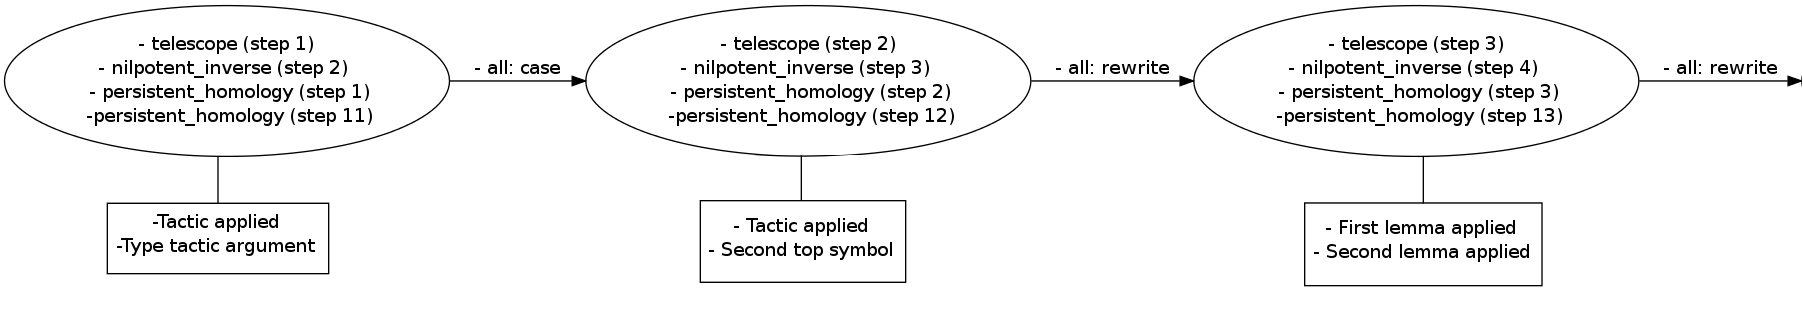
\includegraphics[scale=.19]{itp6.png}
\caption{\scriptsize{\emph{Fragment of the automaton 
 corresponding to the cluster of four lemma fragments described in the case study of Section~\ref{sec:recurrent}} (the whole automaton can be seen in Appendix~\ref{sec:automaton}). 
It shows correspondence between certain proof steps of lemmas % the following lemmas were discovered:
\texttt{telescope} (for the lemma of Example~\ref{example0}), \texttt{nilpotent\_inverse} (for Lemma~\ref{lem:nilpotent2}), and \texttt{persistent\_homology} 
(for Lemma~\ref{lem:fundamental}). Square boxes denote feature correlation where it exists. 
To be compact, we  hide full lemma statements, tactic and auxiliary lemma names, symbols, etc., but they can be shown by ML4PG. 
%For example, the full statements of the following cluster lemmas will be shown:
%The names of the lemmas of that cluster are: 
}}\label{fig:automata}
\end{figure}




\paragraph{A tree representation for terms}

As we have previously explained, ML4PG can cluster terms using a recurrent clustering process (see Section~\ref{sec:reclemmaclustering}). When using this tool, the output generated by ML4PG is a list of names of similar terms, and the user should inspect the libraries to compare the different terms. In order to simplify this process, we have created a visualisation tool that generates the ML4PG term-tree (cf. Definition~\ref{def:ml4pgtermtree}) given the name associated with a term.

\begin{example}
 In Example~\ref{ex:maxnACA}, we have shown how the lemma \lstinline?maxnACA? is automatically proven thanks to its similarity with lemmas \lstinline?addnACA?, \lstinline?minnACA?, \lstinline?mulnACA?. From Figure~\ref{fig:treevisualisation}, it is trivial why these 4 lemmas are similar.

 
 

\begin{figure}
\centering
\begin{tikzpicture}
\draw (0,0) node{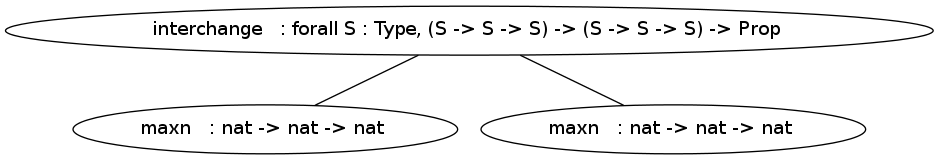
\includegraphics[scale=.2]{maxnACA.png}} ;
\draw (7,0) node{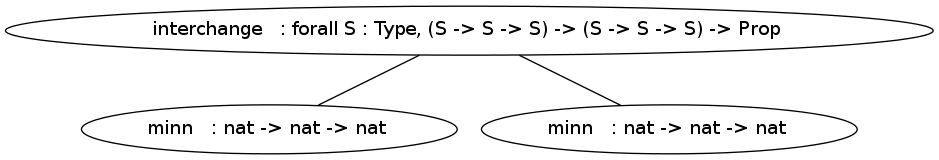
\includegraphics[scale=.2]{minnACA.png}};
\draw (0,-1.5) node{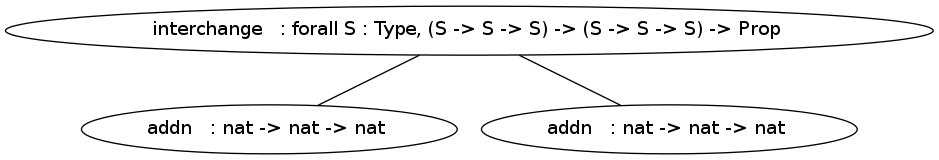
\includegraphics[scale=.2]{addnACA.png}} ;
\draw (7,-1.5) node{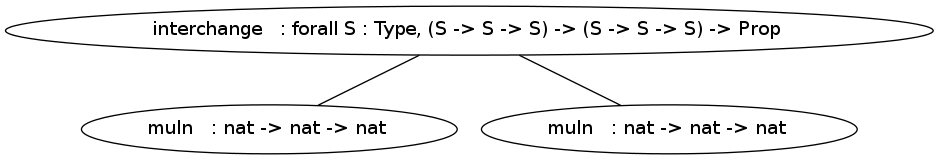
\includegraphics[scale=.2]{mulnACA.png}}  ;
\end{tikzpicture}
\caption{Term trees associated with \texttt{maxnACA} (top left), \texttt{minnACA} (top right), \texttt{addnACA} (bottom left), \texttt{mulnACA} (bottom right).}\label{fig:treevisualisation} 
\end{figure} 
 
 \end{example}

 
\paragraph{Cluster visualisation}

Finally, we have also improved the visualisation of clusters. Initially, ML4PG's output is a list of similar lemmas (or in general terms), and the user can adjust the accuracy of those families varying the granularity value (see the case studied included at the end of Section~\ref{sec:recurrent}). However, this means that he has to run the clustering process several times, and remember the families that were generated in each iteration. These problems have been tackled thanks to a new visualisation tool that captures the relations between the families of similar proofs/terms obtained using different granularity values, see Figure~\ref{fig:clustervisualisation}.




\begin{figure}
\centering
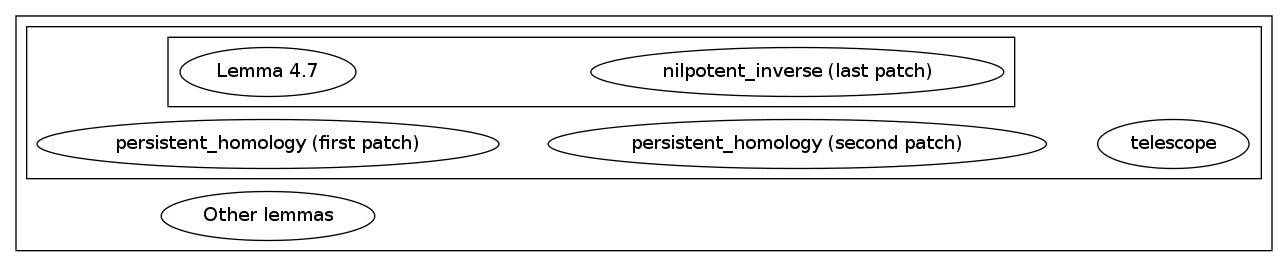
\includegraphics[scale=.3]{clustervisualisation.png}
\caption{Cluster visualisation for the case study included at the end of Section~\ref{sec:recurrent} regarding the families of similar lemmas to Lemma~\ref{lem:nilpotent}: \texttt{telescope} (for the lemma of Example~\ref{example0}), \texttt{nilpotent\_inverse} (for Lemma~\ref{lem:nilpotent2}), and \texttt{persistent\_homology} 
(for Lemma~\ref{lem:fundamental}). The outer, middle and inner square contain, respectively, the proof-patches obtained with granularities 1, 3 and 5. It shows correspondence between certain proof steps of lemmas % the following lemmas were discovered:
}\label{fig:clustervisualisation} 
\end{figure} 



%for clustering that are related to that 
%state.


% $-$ there are several transitions from the $j$th to the $j+1$th state labelled by the $j$th tactic of each proof-patch of $P$ -- if either the $j$th tactic of two or more
% proof-patches is the same or belong to the same group (see Table~\ref{tab:tactics}), the transitions are merged in a unique transition labelled with the set of those tactics,
% 
% $-$ if a proof ends after the $j$th tactic of a proof-patch, the $j+1$ state is represented as final.

%\begin{example}

 
 




%\end{example}




\section{Related Work}\label{sec:relatedwork}

In this section, we compare ML4PG with tools available in Coq and other ITPs, an overview of this comparison is provided in
Table~\ref{tab:comparison}.

\begin{table}
\tbl{\scriptsize{\emph{Comparison of ML4PG with premise-selection methods, Coq's search mechanisms and dependency graphs.}}\label{tab:comparison}}{
\centering
{\scriptsize
 \begin{tabular}{ p{2cm}  p{1.75cm}  p{1.75cm}  p{1.75cm}   p{1.75cm}   p{1.75cm} }
   \toprule
    & Premise Selection & Search & Dependency graphs & Model Inference & ML4PG  \\
		%\hline
		%\hline
  	%	Fib example & No & No &   \alert{Yes} \\
		%	\hline
\midrule
\midrule
\textbf{Method} & Statistical Proof-Premise Selection & Search & Parsing & Model Inference &  Statistical Pattern-recognition \\

\midrule
   \textbf{Goal-oriented?} & Yes  & Yes &  Not necessarily & No & Not necessarily  \\
\midrule
   \textbf{Deterministic?} & No & Yes &Yes  & No & No   \\
\midrule
	\textbf{Visual representation} & No & No  & Yes  & Yes   & Yes \\
\midrule
	\textbf{Covers proofs or terms?} & Both &Terms/types & Both & Proofs  &  Both  \\
\midrule	
			\textbf{Takes into consideration dependencies?} & Yes & No & Yes & Yes  & Yes \\
\midrule
		\textbf{Finds structural similarities beyond concrete syntax?} & No & No & No  & No & Yes  \\
\midrule
	\textbf{Finds structurally similar patterns in proofs?} & No & No & No & No  & Yes  \\
\midrule
  \textbf{Good for proof automation?} & Depend on background theory & No & No & Depend on background theory & Depend on background theory \\
   \bottomrule
		\end{tabular} }}
\end{table}


\paragraph{Statistical Proof-Premise Selection in ITPs} Proof automation in ITPs has been enhanced with the connection of this kind of 
systems with Automated Theorem Provers (ATPs). The workflow of tools like Sledgehammer~\cite{Paulson_threeyears} or HolyHammer~\cite{holyhammer} consists of the following steps: (1) translation of the statement of the theorem (from the ITP format) to a
first order format suitable for ATPs; (2) selection of the lemmas (or premises) that could be relevant to prove a theorem; 
(3) invocation of several ATPs to prove the result; and (4) if an ATP is successful in the proof, reconstruction of the proof in
the ITP from the output generated by the ATP.

An important issue in the above procedure is the premise selection mechanism, especially when dealing with big libraries, since proofs of some results can be infeasible for the ATPs if they receive too many premises. Statistical machine-learning methods have been 
successfully used to tackle this problem in~\cite{UrbanSPV08,K13,holyhammer}. In particular, a classifier is constructed for every 
lemma of the library. Given two lemmas $A$ and $B$, if $B$ was used in the proof of $A$, a feature vector $|A|$  is extracted 
from the statement of $A$, and is sent as a positive example to the classifier $<B>$ constructed for $B$; otherwise, $|A|$ is
used as a negative example to train $<B>$.
Note that, $|A|$  captures statistics of $A$'s syntactic form relative to
every symbol in the library; and the resulting feature vector is a sparse (including up to $10^6$ features).
 After such training, the classifier $<B>$ can predict whether a new lemma $C$ requires 
the lemma $B$ in its proof, by testing $<B>$ with the input vector $|C|$. On the basis of such predictions for all lemmas in the library,  this tool constructs a hierarchy of the premises that are most likely to be used in the proof
of $C$. 

There are several differences between the statistical premise-selection tools and ML4PG:

\begin{itemize}
 \item \emph{Aim:} premise selection tools help the prover, trying to increase the number of goals automatically proved by ATPs, and ML4PG
 assists the user, providing suggestions as proof hints.
 \item \emph{Features:} premise selection tools extract features from first-order formulas translated from the original syntax of the
 theorem prover; on the contrary, ML4PG directly works with Coq's higher-order formulas and proofs. 
 \item \emph{Dependencies:} premise selection tools capture the dependencies of lemmas used in the proof of theorems; ML4PG not only 
 captures these dependencies but also information about, for instance, tactics involved in a proof.
 \item \emph{Machine-learning methods:} Premise selection tools use supervised learning methods, and ML4PG uses unsupervised techniques.
 \item \emph{Proof Automation:} the success of tools like Sledgehammer depends on several aspects: good methods for premise selection,
 availability of a useful background theory, and success of ATPs and the proof reconstruction tool. In the case of ML4PG, the 
 availability of a background theory is also a key aspect for success proof automation, but it also depends on the existence of 
 theorems that required similar proofs. Hence, both tools are only as good as the background theory that was previously developed. \end{itemize}

% As in the case of proof-automation in ML4PG (cf. Section~\ref{sec:evaluation}), tools like Sledgehammer~\cite{Paulson_threeyears} or HolyHammer~\cite{holyhammer} are only as good as the background theory that was previously developed. Therefore, premise selection tools
% can improve the performance of those tools as long as the necessary lemmas are available.


\paragraph{ML4PG vs Coq's Searching Tools} Coq/SSReflect already provides comprehensive search mechanisms to inspect the corpus of results available in different libraries.
There are several search commands in Coq:  \lstinline?Search?~, \lstinline?SearchAbout?, \lstinline?SearchPattern?
and \lstinline?SearchRewrite?~\cite{Coq}. In addition, SSReflect implements its own version of the \lstinline?Search?
command \cite{SSReflect} --- SSReflect's \lstinline?Search? gathers the functionality of the 4 Coq's search commands.
The Whelp platform~\cite{AspertiGCTZ04} is a web search engine for mathematical knowledge formalised in Coq, which features 3 functionalities:
\lstinline?Match? (similar to Coq's \lstinline?Search? command), \lstinline?Hint? (that finds all the theorems which can
be applied to derive the current goal) and \lstinline?Elim? (that retrieves all the eliminators of a given type).
%In this section, we compare ML4PG with these tools.  

%Let us explain first when these tools are usually invoked. 
The existing search mechanisms can be used in two different scenarios. If the user knows how to continue the proof, but
he does not remember (or know) the concrete name of the desired auxiliary lemma, it suffices to provide a search pattern to Coq searching engines, e.g.
using commands of the form
``\lstinline?Search "distr"? \lstinline?in bigop?'' or   
``\lstinline?Search _ (_ * (\big[_/_]_(_ <- _| _) _))?'',
 where \texttt{bigop} is a library, \texttt{"distr"} is a pattern in a lemma name, and  \lstinline? _ (_ * (\big[_/_]_(_ <- _| _) _))?
is a pattern for search.
 
%\begin{example}\label{ex:distr}
% In the proof of Lemma~\ref{lem:nilpotent}, we may want to introduce the term $(1-M)$ inside the sum $\sum_{i=0}^{n-1} M^i$, but 
% if we have no experience with the bigop library of SSReflect, it is likely that we do not know the name of the concrete lemma. 
% The lemma which carries out this task can be find using, for instance, the commands \lstinline?Search "distr" in bigop.? or  
%\lstinline?Search _ (_ * (\big[_/_]_(_ <- _| _) _))?. 
%\end{example}
In the second scenario, the user needs help in the middle of the proof. Searching mechanisms can be also useful in this 
case; for instance, using the \lstinline?Search? command the user can search all the lemmas associated with a concrete term
of the current goal. The \lstinline?Hint? mechanism of Whelp can find all the theorems which can be applied to derive the current goal.

%\begin{example}\label{ex:fact}
% In the proof of Lemma~\ref{lem:factorial}, we can find all the lemmas related to the factorial function using the command
% \lstinline?SearchAbout factorial?. 
%\end{example}

%ML4PG is helpful in the second scenario, since it provides families of similar proofs. Inspecting that family of proofs, 
%the user can find a pattern to finish the proof that she is formalising. 

%As we have seen in Examples~\ref{ex:distr} and~\ref{ex:fact}, 
The above search mechanisms are goal directed and deterministic. That is, the user
searches  the chosen  libraries for lemmas related to a concrete type, term or pattern. 
If the patterns defined by the user are present in the given library, then the user is guaranteed to see the relevant lemmas on the screen.

The situation is more complicated if the user does not know the right pattern to search for. Imagine, for example, being in the middle of constructing a proof, 
and wishing to get some higher-level hint on how to proceed, wishing there was an ITP expert near, who would suggest a further proof strategy based on his previous experience. ML4PG was created to emulate such intelligent help automatically, using statistical machine-learning algorithms to use the information arising from the ``previous experience''.

In comparison to the more traditional \emph{search engines}, ML4PG is a goal-independent (unsupervised) tool, i.e. the user does not have to know the required pattern in advance. But, as many statistical machine-learning applications, it is also non-deterministic. That is, the tool failing to suggest a proof pattern does not mean there is no ``interesting'' pattern to be found. Actually, the notion of a proof pattern being ``interesting'' is left to the user's judgement, as well. 

\paragraph{ML4PG vs Coq's Visualisation Tools} Several visualisation tools have been developed to facilitate the understanding
of the dependencies that arise in Coq developments. Namely, Coq provides tools to visualise dependencies among files, dependencies 
between theorems and definitions, proof-trees, and proof-models.

Large Coq developments involve hundreds of files (e.g. 125 files in the proof of the Feit-Thompson theorem); therefore, the 
computation and visualisation of the dependencies among those files is an important issue to maintain those developments. The 
Coq distribution provides the \lstinline?coqdep? tool to compute file dependencies. The output generated by \lstinline?coqdep? 
can be fed into the tool developed in~\cite{dependtohtml} to visualise file dependencies (see Figure~\ref{fig:depend-files}). 

\begin{figure}[t]
\centering 
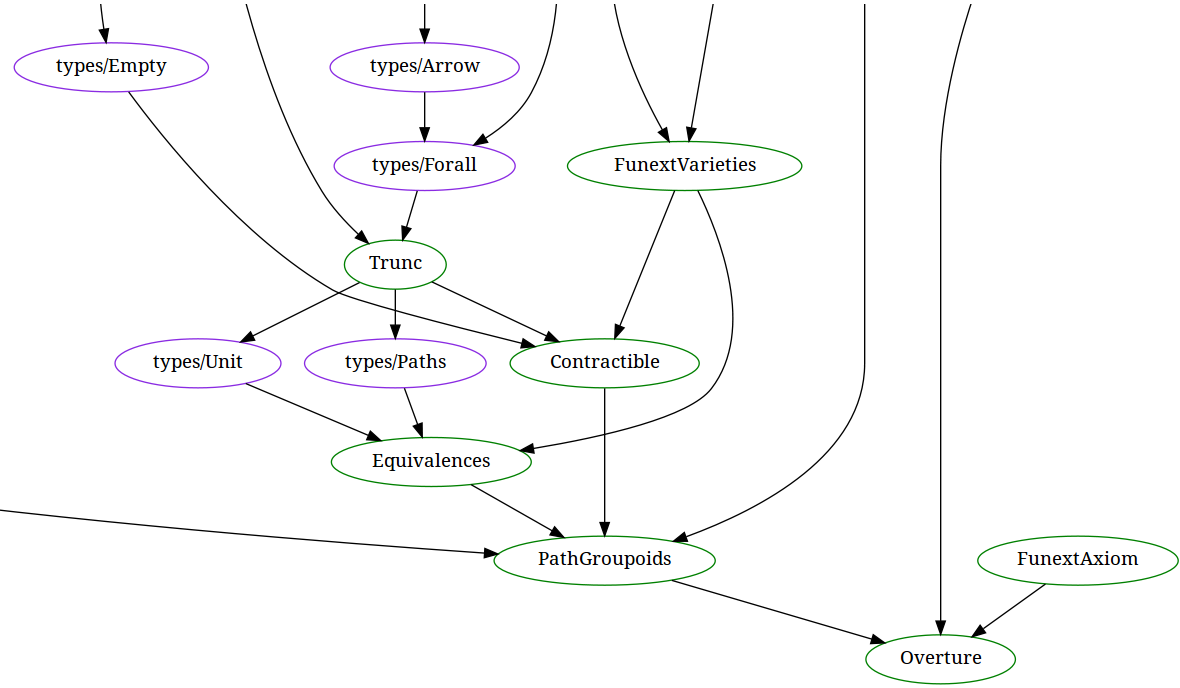
\includegraphics[scale=.4]{HoTTCorefragment.png}
\caption{\scriptsize{\emph{Fragment of the dependency graph of the HoTT library.} The complete dependency graph is available at the HoTT wiki\protect\cite{hottbook}.}}\label{fig:depend-files}
\end{figure}

A different set of tools~\cite{dpdgraph,BPP00} has been developed to compute and visualise dependencies between theorems and definitions, see Figure~\ref{fig:dgraph1}. An analysis of proof terms makes it possible to know whether some theorem is used when proving another result or when defining a new concept. Visualising the complete graph of dependence is useful to detect the results that are not used, and to foresee the impact of modifying a theorem or definition.  

These dependency graphs are designed to, mainly, work with proofs rather than object definitions and do not show the term structure per se,
but only the dependencies between the auxiliary lemmas/constructors used. Moreover, they give a complete information of all the results that were necessary to prove a given lemma, making hard to read them, due to the presence of this complete information. Hence,  statistical machine learning may be useful for data-mining the above information in order to discriminate unimportant features of the
lemma, and highlight those that are important. ML4PG essentially does this. ML4PG's recurrent clustering  captures term and lemma dependencies recurrently, via the feature extraction which itself involves recurrent clustering of all previously
defined terms. 


ML4PG's proof clustering in particular is very close to dependency graphs for lemmas, in that both are capturing mutual or inductive dependencies of all lemmas needed to prove the given statement. As a result, ML4PG can be seen as a post-processing tool for dependency
graphs. Given a big graph as shown in Figure~\ref{fig:dgraph1}, what is the right way to discriminate its unimportant features? How to decide which of them are important or not? One of the ways to do this, is to determine that relatively to other lemmas in the library. This is achieved by applying clustering in ML4PG. Taking all of the above features into account, ML4PG can associate various object definitions
and lemma statements and lemma proofs. 

\begin{figure}
\centering
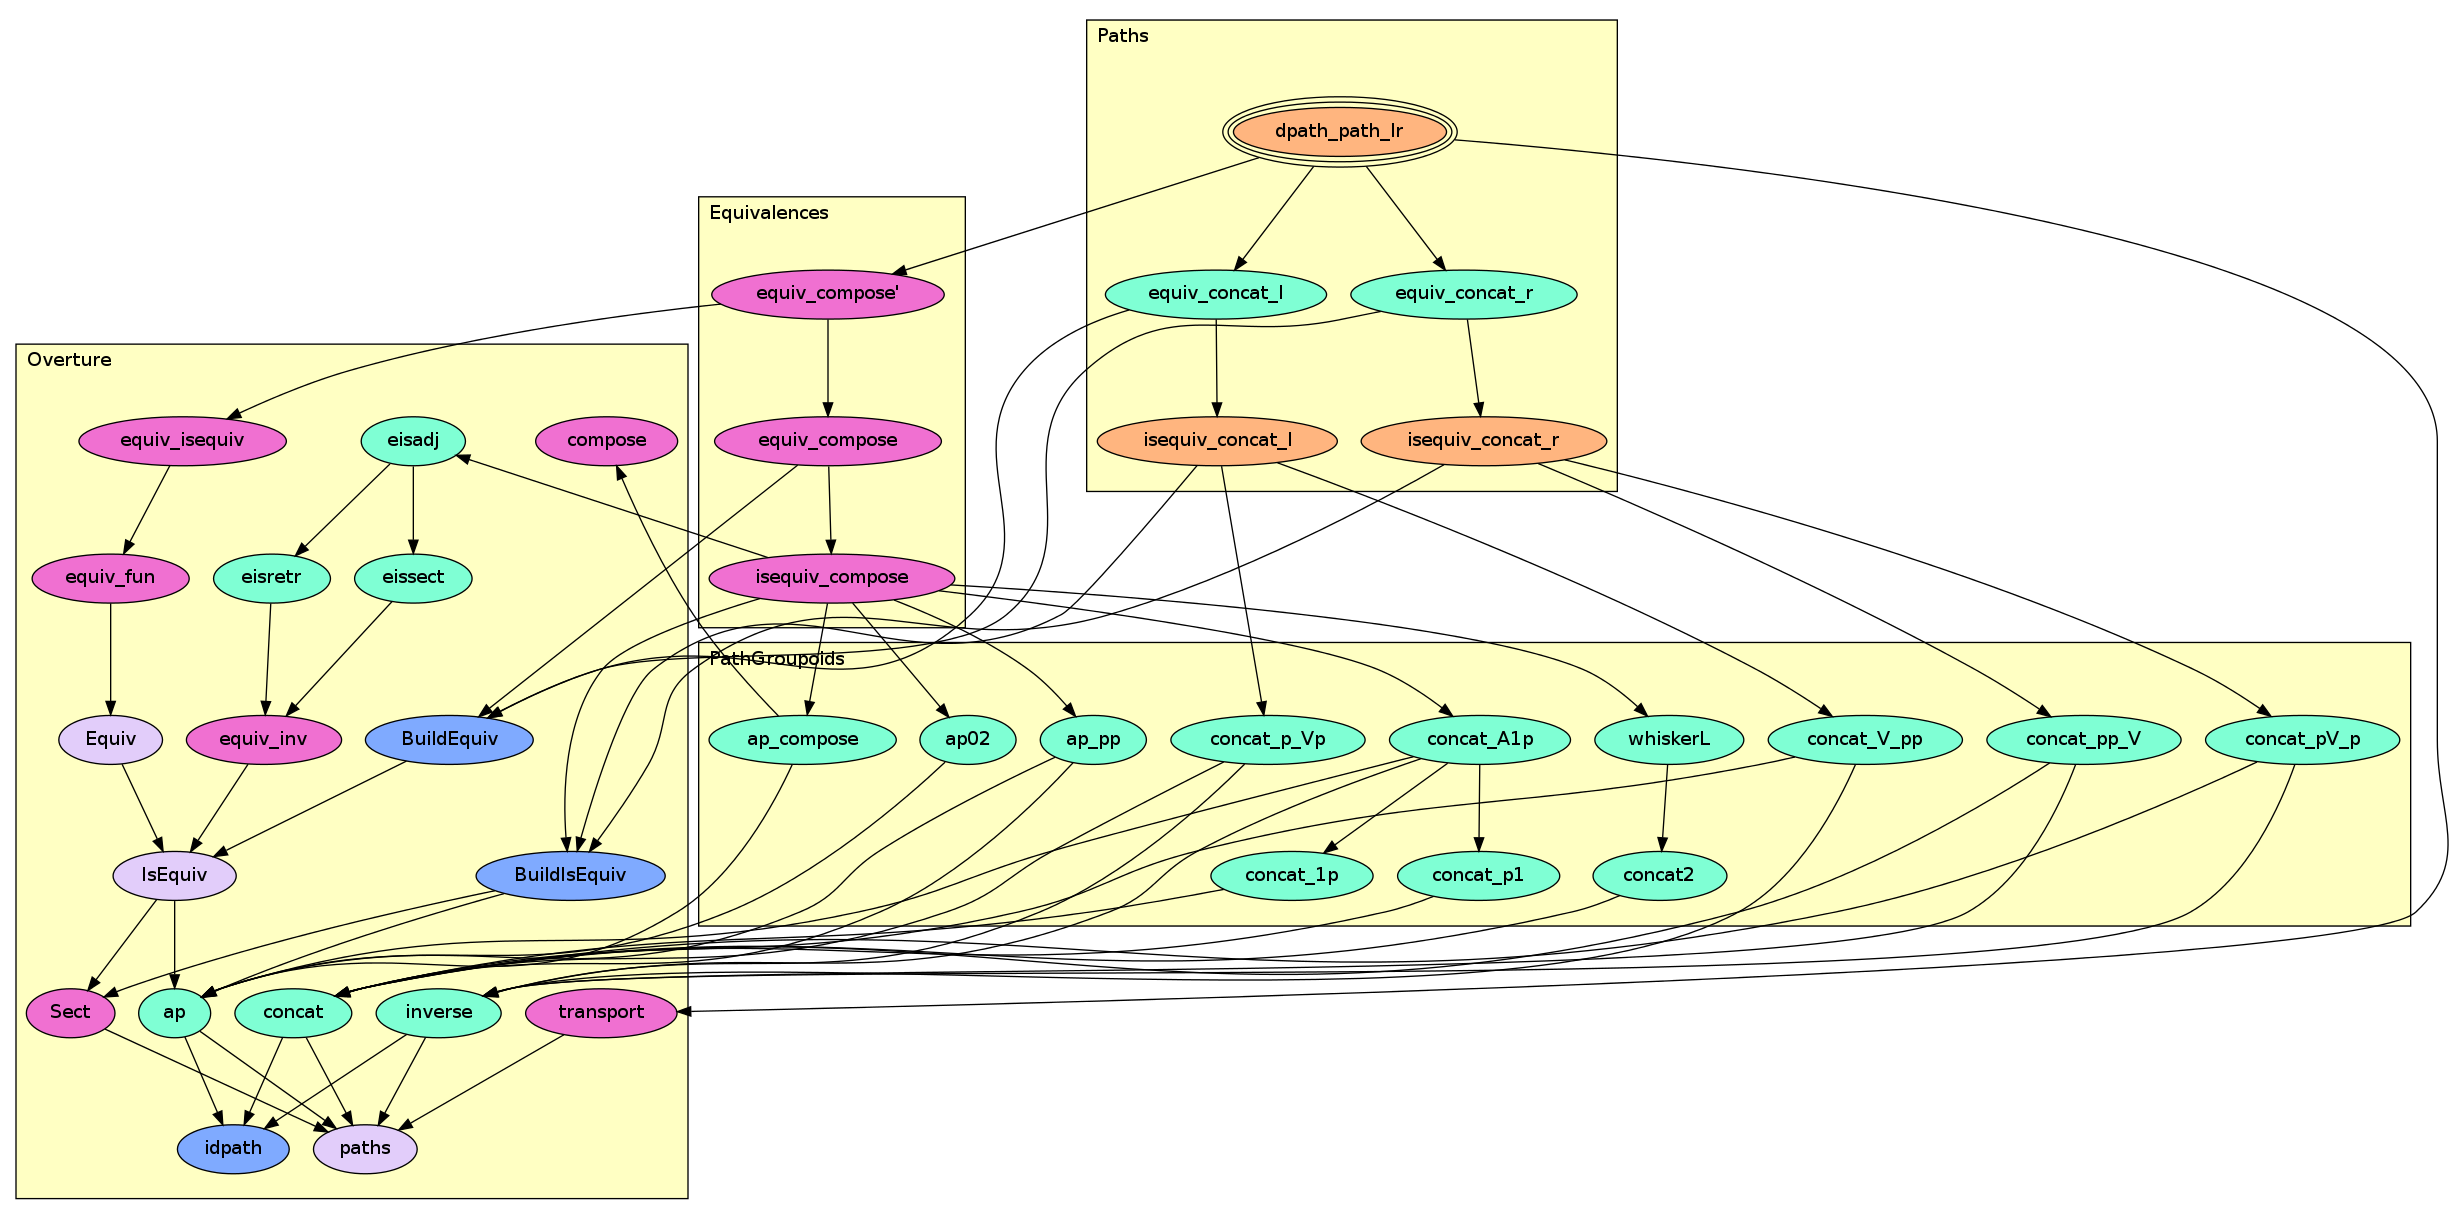
\includegraphics[scale=.15]{graph_dpath_path_lr.png}
\caption{\scriptsize{\emph{Dependency graph for the theorem \texttt{dpath\_path\_lr} included in the \texttt{Paths} library of HoTT.}}}\label{fig:dgraph1}
\end{figure}

The tools presented in~\cite{dpdgraph,BPP00} can also be used to visualise dependency graphs for terms, see Figure~\ref{fig:dgraph2}. 
ML4PG’s term-structure clustering goes beyond these dependency graphs for terms, and carefully captures the tree term shape, structure,
and dependency on other term- and type- structures present in the library (see Figure~\ref{fig:treevisualisation}). ML4PG's approach makes sure that dependency of auxiliary terms/types on other terms/types defined in Coq libraries is taken into account recurrently. 


\begin{figure}
\centering
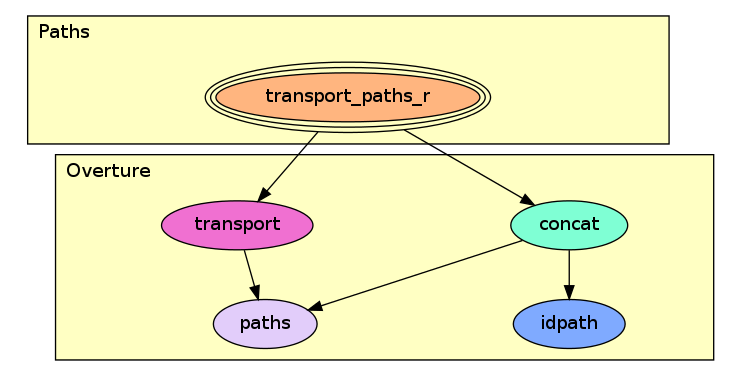
\includegraphics[scale=.35]{graphpaths.png}
\caption{\scriptsize{\emph{Dependency graph for the definition of \texttt{transport\_paths\_r} included in the \texttt{Paths} library of HoTT.}}}\label{fig:dgraph2}
\end{figure}


Coq also supports the visualisation of the proof-tree during an interactive proof development using the Prooftree tool~\cite{prooftree}. This tool was aimed to visualise the different subgoals that arise during the development of a proof, see Figure~\ref{fig:prooftree}. ML4PG automaton representation of proofs (cf. Figure~\ref{fig:automata}) not only shows the applied tactics, but also the generated-subgoals in each step, and compare the proof flow of the current proof with the steps followed in other theorems. 

\begin{figure}
\centering
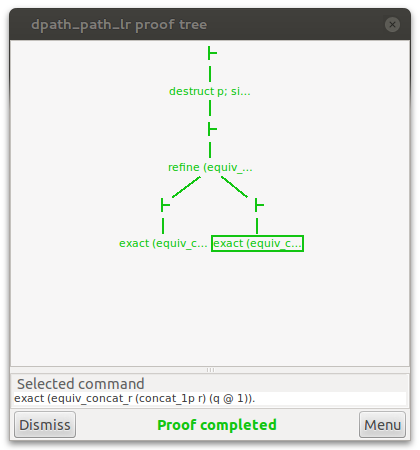
\includegraphics[scale=.5]{prooftree.png}
\caption{\scriptsize{\emph{Proof tree for the theorem \texttt{dpath\_path\_lr} included in the \texttt{Paths} library of HoTT.}}}\label{fig:prooftree}
\end{figure}

Finally, the tool presented in~\cite{GNR14} can infer models from Coq developments. Those models are represented as automata that are latter used to generate proof attempts. Since the models were designed with the aim of automatically generate proofs, they are not human-readable. 
ML4PG's graphical representation of automata is simpler than the work presented in~\cite{GNR14}.  







\section{Conclusions}\label{sec:conclusions}

We have presented several enhancements of the ML4PG system. \emph{Term clustering} adds a new
functionality to ML4PG: the user can receive suggestions about families of similar definitions, types and lemma shapes (in fact, any Coq terms).
The \emph{proof-patch method} is employed to analyse the properties of the patches that constitute a proof. The whole syntax of Coq libraries is now subject to \emph{recurrent clustering}, which
 increases the number and accuracy of families of similar proofs suggested by ML4PG. In addition, this information is taken into account in an automatic proof-generation method. Finally, the different visualisation tools implemented in ML4PG facilitates the interpretation of clusters of similar proof-patches and terms.

Further improvements in \emph{accuracy} (e.g. including proof contexts into the analysis) and \emph{conceptualisation} for clustered terms and proofs are planned. The families of similar proofs and terms can be the basis to
apply symbolic techniques to, for instance, infer models from proof traces~\cite{GNR14}, or generate auxiliary results using
mutation of lemmas~\cite{lpar13}. We expect that the incorporation of these techniques help in the goal pursued by ML4PG: make the
proof development easier.















\bibliographystyle{ACM-Reference-Format-Journals}
\bibliography{biblio}

\pagebreak

\appendix

\section{Formula for Gallina tokens}\label{sec:gallinasyntax}


We split Gallina tokens into the following groups.

\begin{itemize}
 \item Group 1: \lstinline?forall?, \lstinline?->?.
 \item Group 2: \lstinline?fun?,
 \item Group 3: \lstinline?let?, \lstinline?let fix?, \lstinline?let cofix?.
 \item Group 4: \lstinline?fix?, \lstinline?cofix?.
 \item Group 5: \lstinline?@?,
 \item Group 6: \lstinline?match?, \lstinline?if?.
 \item Group 7: \lstinline?:=?, \lstinline?=>?, \lstinline?is?. 
 \item Group 8: \lstinline?Inductive?, \lstinline?CoInductive?.
 \item Group 9: \lstinline?exists?, \lstinline?exists2?.
 \item Group 10: \lstinline?:?, \lstinline?:>?, \lstinline?<:?, \lstinline?%?.
 
 
\end{itemize}



The formula for the $j$th Gallina token of the $n$th group is given by the formula $$- (n + \sum_{i=0}^j \frac{1}{10\times 2^{i-1}})$$




\newpage

\section{Groups of Coq tactics and number assignment}\label{sec:coqtactics}

% We have divided the Coq tactics in the groups presented in Table~\ref{tab:coqtactics}.

Table~\ref{tab:coqtactics} splits the Coq tactics into different groups. The formula used in the function $[.]_{tactic}$ 
to compute the value of a Coq tactic is given by 
$i+\sum_{j=0}^k\frac{1}{10 \times 2^{j-1}}$ where $i$ is the group of the tactic and $k$ is the position 
of the tactic in that group (cf. right side of Table~\ref{tab:coqtactics}). 

\begin{table}[h]
\tbl{{\scriptsize \emph{Groups of Coq tactics}}\label{tab:coqtactics}}{
\centering
\begin{tabular}{l||l}

Group & Tactics of the group\\

\hline
\hline
Group 1:           &  \lstinline?exact, eexact, assumption, eassumption, ?\\
Applying theorems &  \lstinline?refine, apply, eapply, simple apply, lapply, ?\\
\hline
Group 2:           &  \lstinline?constructor, split, exists, left, right, ?\\
Managing inductive constructors & \lstinline?econstructor, esplit, eexists, eleft, eright?\\
\hline
Group 3:           &  \lstinline?intro, intros, clear, rever, move, rename,  ?\\
Managing local context & \lstinline?set, remember, pose, decompose?\\
\hline
Group 4:            &  \lstinline?assert, cut, pose, specialize, generalize, ?\\
Controlling proof flow & \lstinline?evar, instantiate, admit, absurd, ?\\
& \lstinline?contradition, contradict, exfalso?\\
\hline
Group 5:            & \lstinline?destruct, case, ecase, simple destruct,?\\
Case analysis and induction & \lstinline?induction, einduction, elim, eelim, ?\\
 & \lstinline?simple induction, double induction, ?\\
     & \lstinline?dependent induction, functional induction,?\\
  & \lstinline? discriminate, injection, fix, cofix, ?\\
    & \lstinline? case_eq, elimtype?\\
\hline
Group 6:          &  \lstinline?rewrite, erewrite, cutrewrite, replace, ?\\
Rewriting expressions &  \lstinline?reflexivity, symmetry, transitivity, subst, ?\\
&  \lstinline?stepl, change?\\
\hline
Group 7:          &  \lstinline?cbv, compute, vm_compute, red, hnf, simpl, ?\\
Performing computations  &  \lstinline?unfold, fold, pattern, conv_tactic?\\
\hline
Group 8:           &  \lstinline?auto, trivial, eauto, autounfold, ?\\
Automation       &  \lstinline?autorewrite?\\
\hline
Group 9:           &  \lstinline?tauto, intuition, rtauto, firstorder, ?\\
Decision procedures & \lstinline?congruence?\\
\hline
Group 10 &  \lstinline?decide equality, compare, simplify_eq,?\\
Equality & \lstinline?esimplify_eq?\\
\hline
Group 11 &  \lstinline?inversion, dependent inversion,?\\
Inversion & \lstinline?functional inversion, quote?\\
\hline
Group 12 & \lstinline?classical_left, classical_right?\\
Classical tactics & \lstinline??\\
\hline
Group 13 & \lstinline?omega, ring, field, fourier?\\
Automatizing & \\
\hline
Group 14 & Rest of Coq tactics\\
\hline
\end{tabular}}
\end{table}





\newpage




\section{Automaton}\label{sec:automaton} 
 
 

\begin{figure}[h]
    \centering
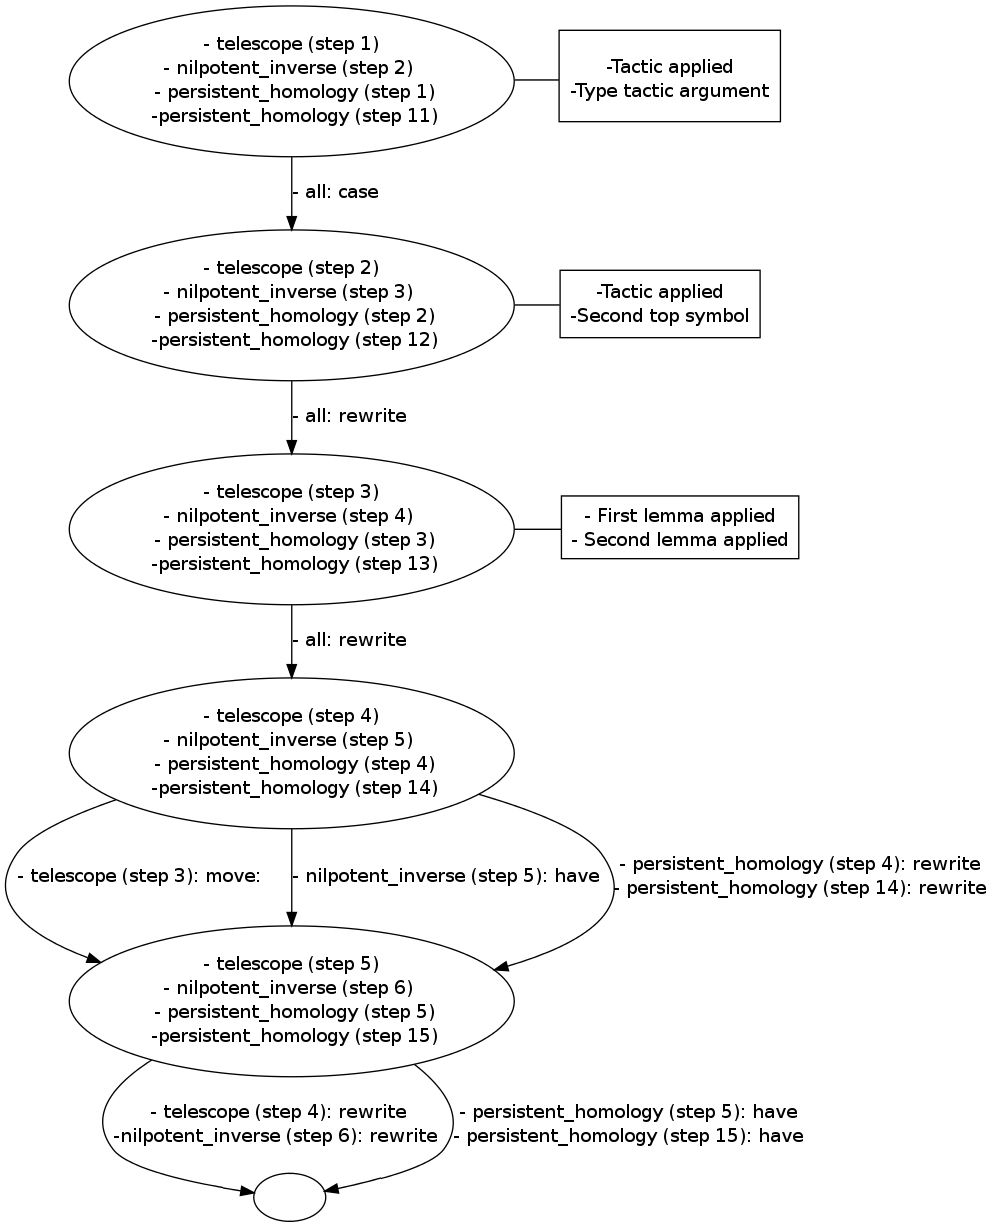
\includegraphics[scale=0.28]{itp.png} 
\caption{\scriptsize{\emph{Automaton corresponding to the proof cluster of four lemma fragments described in the case study of Section~\ref{sec:recurrent}.} The automaton shows the five proof steps, of which the first three are shown to influence the cluster formation.
It uses Lemma names: \texttt{telescope} for the lemma of Example~\ref{example0}, \texttt{nilpotent\_inverse} for Lemma~\ref{lem:nilpotent2}, and \texttt{persistent\_homology} 
for Lemma~\ref{lem:fundamental}.
  In addition to Lemma names, ML4PG can show lemma statements, and it can provide details of the \lq\lq{}Tactic applied\rq\rq{}, \lq\lq{}Type tactic argument\rq\rq{}, \lq\lq{}Second top symbol\rq\rq{}, \lq\lq{}First/Second lemma applied\rq\rq{} fields.}}
\end{figure}






\end{document}
